\documentclass{beamer}

% Theme and packages
\usepackage{subcaption}
\usepackage{hyperref}
\usepackage{threeparttable}
\usepackage{longtable} 
\usepackage{booktabs} % for \cmidrule
\usepackage{array}
\usepackage{natbib}
\usepackage{etoolbox}
\setlength{\bibsep}{0pt plus 0.3ex}
\usetheme{Warsaw}
\usecolortheme{seahorse}
% \setbeamertemplate{frame numbering}[fraction]
\useoutertheme[subsection=false]{miniframes}
\setbeamercolor{title page}{bg=white}
% \setbeamertemplate{footline}[frame number]
\setbeamertemplate{footline}{
    \leavevmode%
    \hbox{%
        \begin{beamercolorbox}[wd=0.7\paperwidth,ht=2.5ex,dp=1.5ex,left]{author in head/foot}%
            \hspace{1em}\insertshortauthor{} -- \insertshorttitle{}
        \end{beamercolorbox}%
        \begin{beamercolorbox}[wd=0.3\paperwidth,ht=2.5ex,dp=1.5ex,right]{author in head/foot}%
            \insertframenumber{} \hspace{1em}
        \end{beamercolorbox}%
    }
}  

% Title, author, and date information
\title[Effects of Local Road Tax Cuts]{The Effect of Local Road Maintenance Tax Cuts on House Values}
\subtitle{Joint work with David Brasington}
\author{Saani Rawat}
\institute[UC / AREUEA]{University of Cincinnati \\ AREUEA National Conference 2025}
\date{May 29, 2025}

\begin{document}

% Title page
\begin{frame}
    \titlepage
\end{frame}

% Outline slide
\begin{frame}{Outline}
    \tableofcontents
\end{frame}
 
%-------------------------------------------------------
% Section 1: Introduction
%-------------------------------------------------------
\section{Introduction}

\begin{frame}{Research Question}
    \begin{itemize}
        \item \textbf{Primary Question:} What is the impact of local road maintenance tax cuts on house values?
        \item Local road maintenance in Ohio funded by \textbf{road tax levies} that are up for renewal every 5 years
    \end{itemize}

    \begin{figure}[ht]
        \centering
        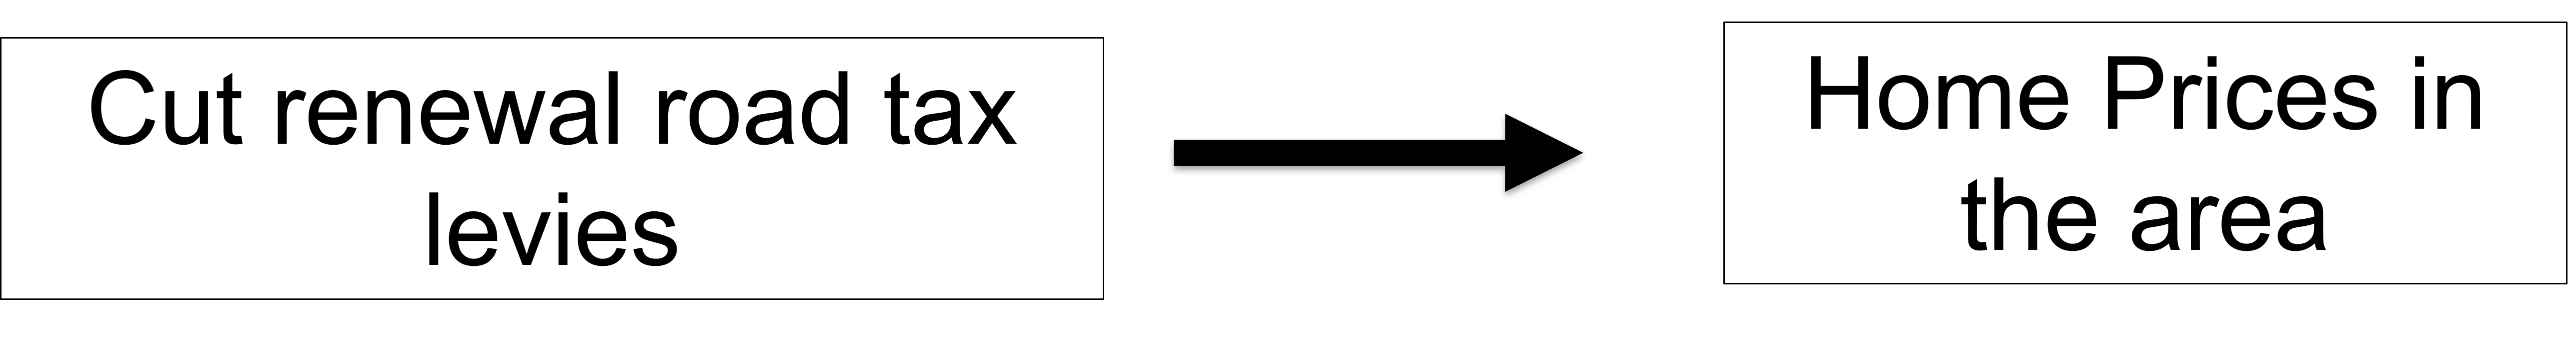
\includegraphics[width=0.8\textwidth]{images/research_question.png}
        \label{fig:research_question}
    \end{figure}
\end{frame}

\begin{frame}[label=who_funds_roads]{Background}
    Who funds the roads in Ohio?
    \begin{itemize}
        \item {Federal Government: } New project grants by FHWA
        \item {State Government: } Inter-state highways and arterial roads
        \item {\bf \underline{Local Governments:}} Local roads 
    \end{itemize}

    \begin{flushright}
        \hyperlink{odot_who_does_what}{\beamergotobutton{ODOT Source}}
    \end{flushright}

    How are roads funded in Ohio?
    \begin{itemize}
        \item {Gas taxes:} Federal (\$0.18 per gallon) and state (\$0.38 per gallon)
        \item {User taxes:} Licensing, registration fees, tolls etc.
        \item {\bf \underline{Property taxes:}} unvoted (10-mill rule) and \textcolor{red}{\bf voted} (road tax levies - must be approved by residents) 
    \end{itemize}
\end{frame}

\begin{frame}{Local Road Taxation in Ohio}
    \begin{itemize}
        \item 88 counties: Divided in townships, villages and cities %- local governments
        % \item Property tax collected by County Tax Assessor, distributed by county to local governments
        % \item Ohio Revised Code has a 10-mill (1\%) limit on unvoted levies. Additional property tax must be voted upon, and are {\bf approved} or {\bf rejected} by the residents
        % \item Property tax is on assessed value, which is 35\% of appraised value of the property
        \item \textbf{Road tax levies} are a specific-purpose property tax levied by local governments to fund road maintenance, voted on by residents 
        \item These levies expire after 5 years and must be \textbf{\underline{renewed}} by the residents before these taxes can be collected again
        % \item We focus on \textbf{renewal} road tax levies, which avoids endogeneity
        \item Example of a typical levy:

        2-mill (0.2\%), 5-year renewal road tax levy in Adams Township in 1995
    \end{itemize}
\end{frame}

\begin{frame}{Mechanism}
    \begin{itemize}
        \item Renewal tax levy failures reduce road maintenance funding
        \item Loss of maintenance funds contributes to poor road quality
        \item Road quality decline is reflected in house prices
    \end{itemize}
    \begin{figure}[ht]
        \centering
        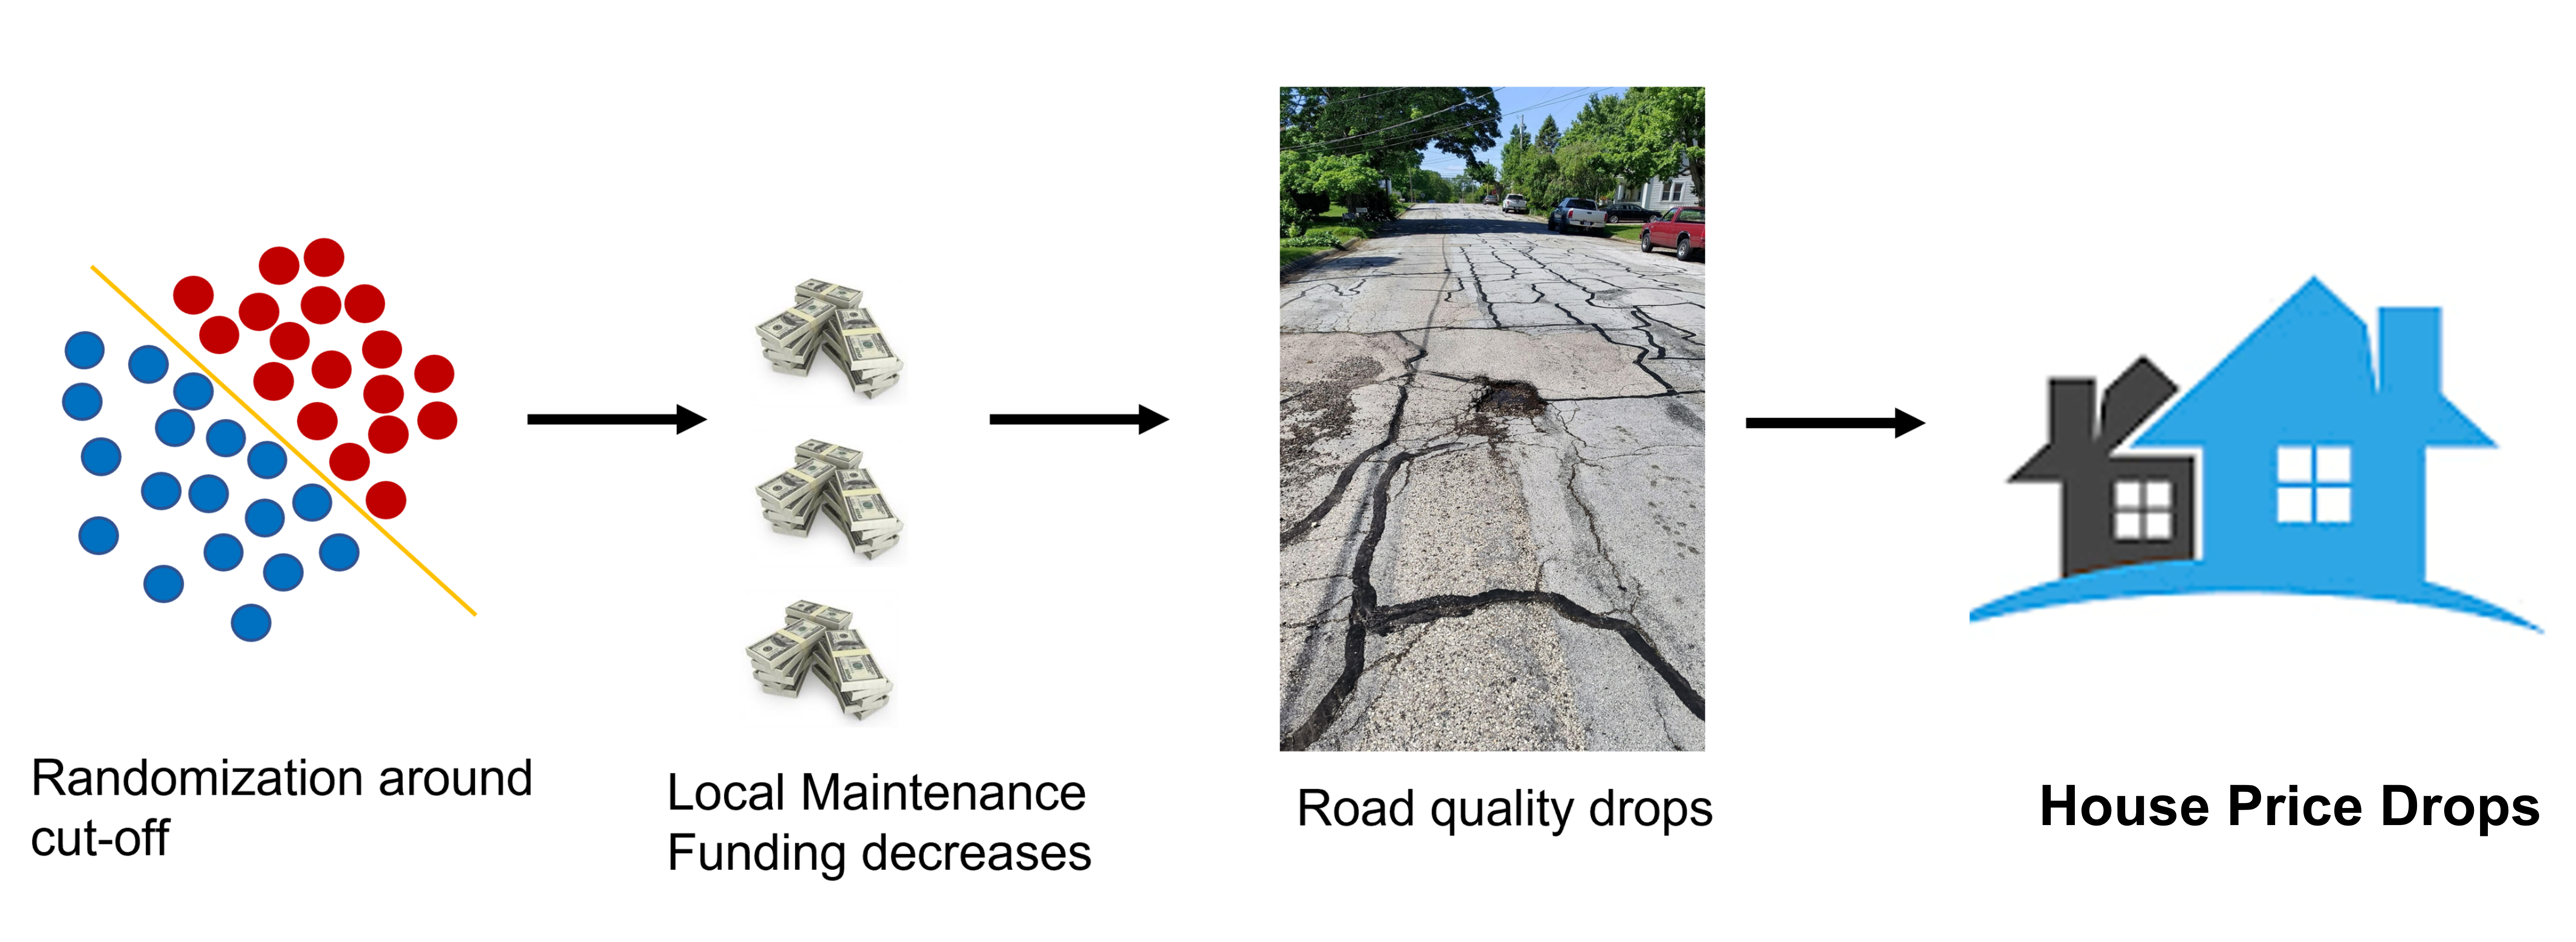
\includegraphics[width=0.8\textwidth]{images/approach.png}
        \caption{How do road tax cuts affect house prices?}
        \label{fig:approach}
    \end{figure}
\end{frame}

\begin{frame}{Contribution}
    \begin{itemize}
        \item We fine-tune GPT-4o vision model to classify road quality from satellite images
        \item We provide empirical estimates and emphasize the role of \textbf{maintaining infrastructure} in a \textbf{developed} economy
        \item Focus on \textbf{long-term impacts} of cutting a specific-purpose tax on house values
    \end{itemize}
\end{frame}

%-------------------------------------------------------
% Section 2: Literature Review & Data
%-------------------------------------------------------
\section{Lit Review \& Data}

\begin{frame}[label=lit1]{Literature Review}
    \begin{itemize}
        \item \textbf{How new infrastructure impacts house prices:} 
        \begin{itemize}
            \item \cite{hoogendoorn2019house}, \cite{li2016wheels}, \cite{gibbons2005valuing}, \cite{levkovich2016effects}, \cite{beenstock2016hedonic}
        \end{itemize}
        \vskip 0.5cm
        \item \textbf{How maintenance impacts house prices:} \cite{edel1974taxes}, \cite{rioja2003}
        \vskip 0.5cm
        \item \textbf{How roads affect daily lives:} 
        \begin{itemize}
            \item \cite{currier2023}, \cite{asher2020}, \cite{adukia2020}, \cite{gibbons2019new}, \cite{hettige2006}
        \end{itemize}        
        \vskip 1cm
        \begin{flushright}
            \hyperlink{gdp_and_roads}{\beamergotobutton{Roads and GDP per Capita}}
        \end{flushright}        
    \end{itemize}
\end{frame}

\begin{frame}{Literature Review}
    \begin{itemize}
        \item {\bf Roads and House Prices:} \cite{gonzalez2016paving}, \cite{chaurey2022}
        \item \textbf{Identification}: RD \citep{cellini2010value,asher2020}, Randomization \citep{gonzalez2016paving} 
        \item \textbf{Local elections and referendums:} 
        \begin{itemize}
            \item \cite{cellini2010value}, \cite{biasi_what_2025}
        \end{itemize}
        \item \textbf{Method: Dynamic RD estimator}
        \begin{itemize}
            \item \cite{cellini2010value}
        \end{itemize}
        \item {\bf \citeauthor{Oates1972} Decentralization Theorem (1972)} suggests that local governments are better suited to provide local public goods, such as road maintenance, than higher levels of government.
    \end{itemize}
\end{frame}

\begin{frame}{Data Sources}
    \begin{itemize}
        \item \textbf{Local Election Results:} Ohio Secretary of State
        \vskip 0.5cm
        \item \textbf{Housing Prices:} CoreLogic
        \vskip 0.5cm
        \item \textbf{Spending Data:} Audited Financial Reports from Ohio Auditor of State 
        \vskip 0.5cm
        \item \textbf{Road Images:} \textit{\cite{brewer2021} Satellite images dataset}, Google Earth, Google Maps Streetview API, \citeauthor{kaya2024n} (2022, 2024) street images
    \end{itemize}
\end{frame}

%-------------------------------------------------------
% Section 3: Identification Strategy
%-------------------------------------------------------

\section{Identification}

\begin{frame}{Research Design - idea}    
    \begin{figure}[ht]
        \centering
        \begin{subfigure}{0.49\textwidth}
            \centering
            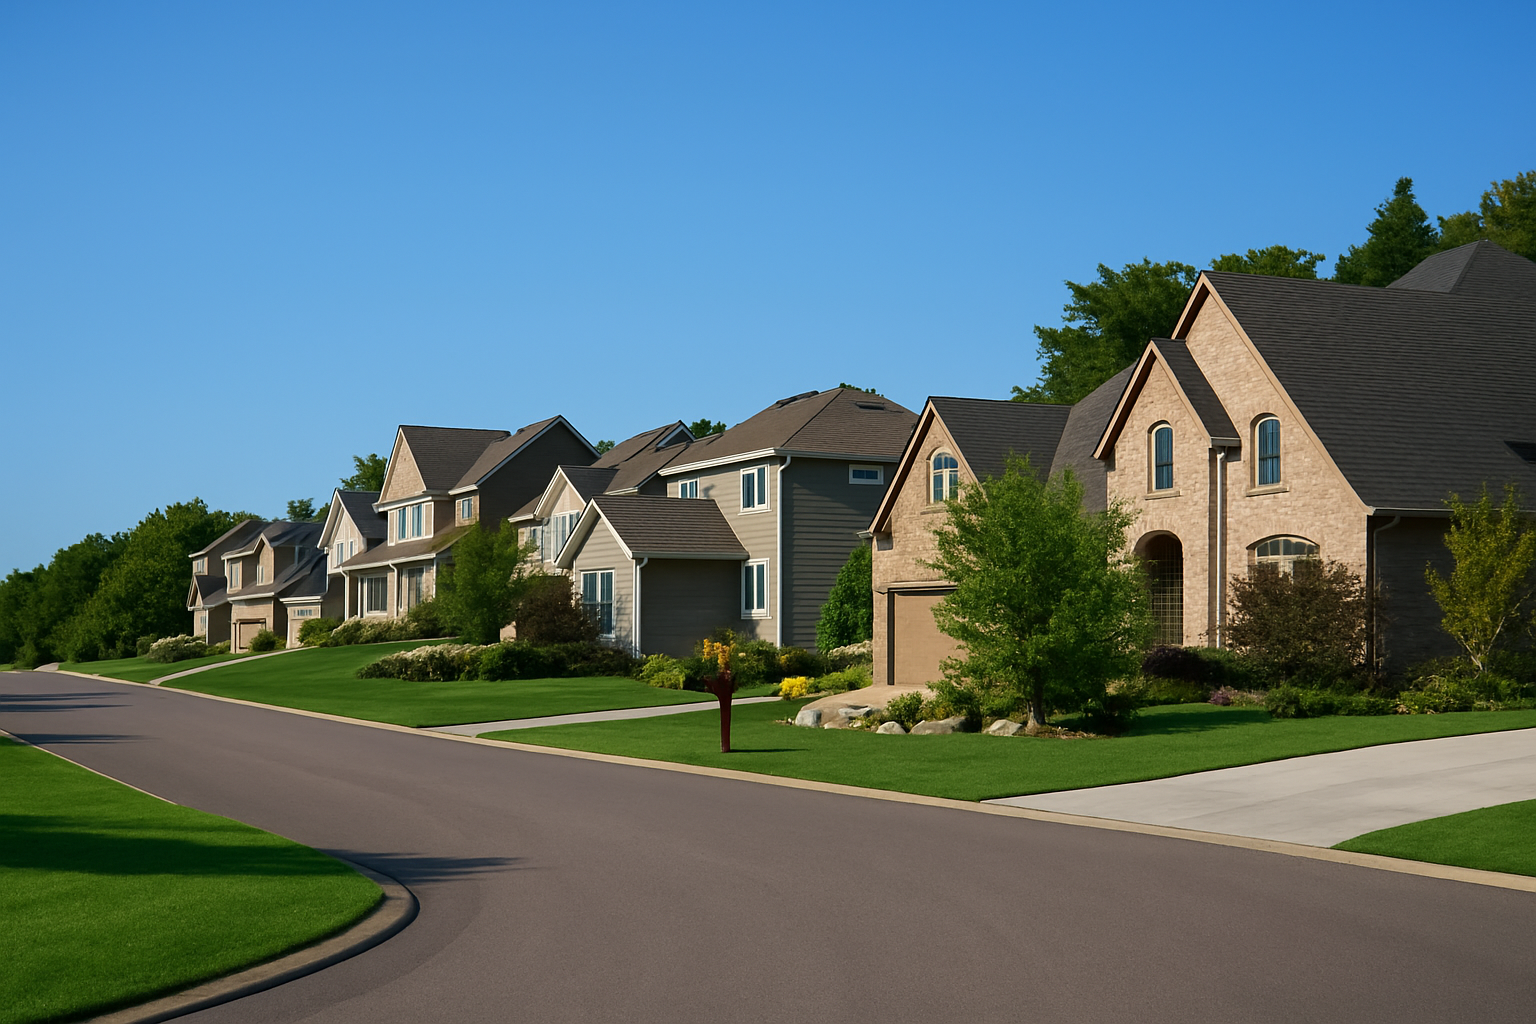
\includegraphics[width=\textwidth]{images/houses_good_roads_ai.png}
            \caption{Houses with good roads}
            \label{fig:good_roads}
        \end{subfigure}
        \hfill
        \begin{subfigure}{0.49\textwidth}
            \centering
            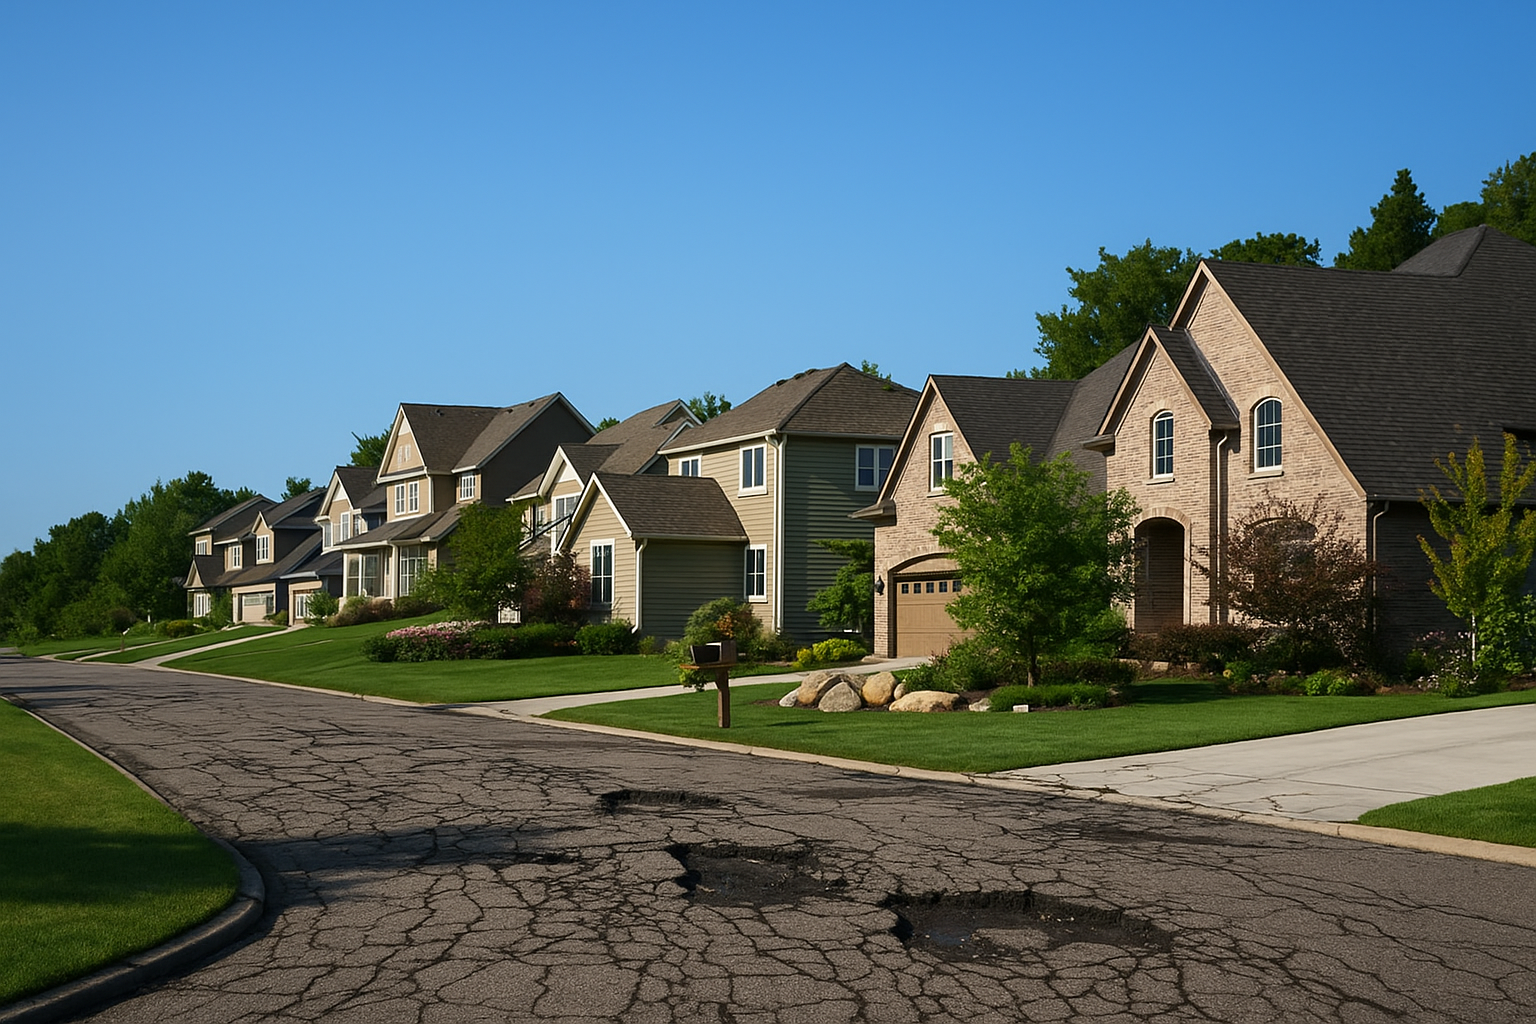
\includegraphics[width=\textwidth]{images/houses_bad_roads_ai.png}
            \caption{Houses with bad roads}
            \label{fig:bad_roads}
        \end{subfigure}
        \caption{Comparing similar neighborhoods and only accounting for differences in roads}
        \label{fig:road_comparison}
    \end{figure}
\end{frame}

\begin{frame}{Running variable: \% votes against the renewal tax levy}
    \begin{itemize}
        \item Before a ``renewal road tax levy'' can be renewed, it must be \textcolor{red}{voted} upon and approved by the residents. These elections are held every 5 years, i.e., residents vote on whether they would like to be taxed or not.
        \item We use the \textbf{percent of votes against} the renewal tax levy as the running variable.
        \item $F_{it}$ is defined as:
            \begin{equation*}
                F_{it} = 
                \begin{cases}
                    1 & \text{, if percent of votes against} > 50\% \ (\text{tax is cut}) \\
                    0 & \text{, if percent of votes against} \leq 50\% \ (\text{tax is renewed})
                \end{cases}
            \end{equation*}
    \end{itemize}
    \begin{flushright}
        \href{https://www.beavercreektwpohio.gov/319/Renewal-Road-Levy}{\beamergotobutton{Renewal proposal example}}
        \href{https://www.cleveland.com/community/2020/11/south-euclid-voters-approve-road-levy-renewal-mayfield-village-residents-pass-four-cleanup-issues.html}{\beamergotobutton{Renewal results example}}
    \end{flushright}
\end{frame}

\begin{frame}{Identification Strategy}
    We use a dynamic \textbf{Dynamic Regression Discontinuity (RD)} design and operationalize CFR (2010)-inspired estimator using the following equation-
        \begin{equation} 
            Y_{i,t+\tau} = \alpha_\tau + \kappa_t + F_{it} {\color{red}{\theta_{\tau}^{ITT}}} + P_g (v_{it}, \gamma_\tau) + Z_{it} \beta_\tau + \epsilon_{i,t + \tau}
            \label{eq:itt_estimator}
        \end{equation}
        \begin{itemize}
            \item[] \scriptsize $Y_{i,t+\tau}$: Outcome variable for city $i$ at year $t + \tau$.
            \item[] \scriptsize $F_{it}$: Indicator variable representing the failure of a city, village, or township to renew its road maintenance tax levy.
            \item[] \scriptsize ${\color{red}{\theta_{\tau}^{ITT}}}$: Causal effect of failing to renew the road tax levy on the outcome.
            \item[] \scriptsize $P_g (v_{it}, \gamma_\tau)$: Polynomial function of the running variable $v_{it}$, which is the percent of votes against the renewal tax levy.
            \item[] \scriptsize $\alpha_\tau$: Timing-specific fixed effects.
            \item[] \scriptsize $\kappa_t$: Year-specific fixed effects.
            \item[] \scriptsize $Z_{it}$: Vector of control variables, including city-level demographics, economic conditions, and other relevant covariates.
            \item[] \scriptsize $\epsilon_{i,t + \tau}$: Error term capturing unobserved factors.
        \end{itemize}
\end{frame}

%-------------------------------------------------------
% Section 4: Spending Measures
%-------------------------------------------------------
\section{Spending Measures}

\begin{frame}
    \begin{center}
        \vspace{2cm}
        {\LARGE \textbf{Spending Measures}}
    \end{center}
\end{frame}

\begin{frame}[label=spending_measures]{Spending Measures}
    \begin{itemize}
        \item \textbf{Metric 1:} Expected loss in road maintenance funds
        \vskip 0.2cm
        
         Loss $=$ Avg Millage Rate $\times$ 0.35 $\times$ Avg. Appraised Value $\times$ \# Households

         \vskip 0.5cm
        \item \textbf{Metric 2:} Spending regression on Road Tax cuts
        $$ Spending = f(Tax \ Cuts)$$
    \end{itemize}
    \begin{flushright}
        \hyperlink{spending_measure_2}{\beamergotobutton{Work on Metric 2}}
    \end{flushright}           
\end{frame}

\begin{frame}{Spending measures: Metric 1 results}
    \begin{table}[ht]
        \centering
        \caption{Spending impact of failing to renew a Road Tax Levy}
        \label{tab:levy_stats}
        \begin{threeparttable}
        \begin{tabular}{p{4.5cm}ccc}
        \hline\hline
        & \textbf{Aggregate} & \textbf{Renewed} & \textbf{Cut} \\
        \hline
        \textbf{Panel A: road tax per household} \\
        Mean & 76 & 75 & 79 \\
           & (55) & (53) & (62) \\
        \hline
        \textbf{Panel B: road tax per city} \\
        Mean & 167,011 & 167,648 & 163,547 \\
           & (340,268) & (340,628) & (338,671) \\
        \hline\hline
        \end{tabular}
        \begin{tablenotes}[flushleft]
          \footnotesize
          \item \textit{Notes:} 
          This table presents descriptive statistics for two measures of the money collected via road tax levies. 
          \textbf{Panel A} reports the mean and standard deviation (SD) of the road tax per household per year. 
          \textbf{Panel B} reports the mean and SD of the total road tax collected per city. 
          “Aggregate” denotes the full sample, while “Renewed” and “Cut” refer to levies that were renewed and failed to renew respectively.
        %   All monetary values are in constant 2010 U.S. dollars and rounded to the nearest integer.
        \end{tablenotes}
        \end{threeparttable}
    \end{table}    
\end{frame}

%-------------------------------------------------------
% Section 5: Road Quality
%-------------------------------------------------------
\section{Road Quality}

\begin{frame}
    \begin{center}
        \vspace{2cm}
        {\LARGE \textbf{Road Quality}}
    \end{center}
\end{frame}

\begin{frame}[label=road_quality_measures]{Road Quality Measures}
    \begin{itemize}
        \item \textbf{Existing Metrics:}
            \begin{itemize}
                \item Road Roughness Index: \cite{currier2023}
                \item International Roughness Index (IRI)
                \item Pavement Condition Rating (PCR) by ODOT
            \end{itemize}        
        \item \textbf{Our Metric:}
            \begin{itemize}
                \item Road Quality Rating: High, Medium, Low
                \item Road Quality Score: 1-100
            \end{itemize}                
        \item \textbf{Satellite-based approach:}
            \begin{itemize}
                \item Using labeled data from \cite{brewer2021}
                \item Fine-tune GPT-4o vision model by OpenAI for road quality classification
                \item Collect Ohio images from Google Earth
                \item Compare \textbf{pre- vs. post-election} images in the same localities
            \end{itemize}
        % \item \textbf{Street-view images approach:}
        %     \begin{itemize}
        %         \item Use \cite{kaya2024n} labeled dataset
        %         \item Leverage Google Streetview API for collecting Ohio images
        %         \item Compare \textbf{pre- vs. post-election} images in the same localities
        %     \end{itemize}
    \end{itemize}
    \begin{flushright}
        \hyperlink{streetview}{\beamergotobutton{Streetview Images Metric}}
        \hyperlink{rqs}{\beamergotobutton{Road Quality Score}}
    \end{flushright}
\end{frame}

% \begin{frame}{Road Quality, Method 1: Satellite images}
%     \begin{itemize}
%         \item \cite{brewer2021} provides 53,000 labeled Satellite Images of roads in U.S.
%         \item They use Google’s Inception V3 ML model to classify road quality into 3 categories:
%             \begin{itemize}
%                 \item 0 for "Low" quality road
%                 \item 1 for "Medium" quality road
%                 \item 2 for "High" quality road
%             \end{itemize}
%         \item We use their images to fine-tune GPT-4O model by Open AI. This multi-modal model has Vision capabilities, meaning it can “see” things and infer
%     \end{itemize}
% \end{frame}

% \begin{frame}[label=brewer_training]{Road Quality: Brewer's Training Data}
%     \begin{figure}[ht]
%         \centering
%         \begin{subfigure}{0.32\textwidth}
%             \centering
%             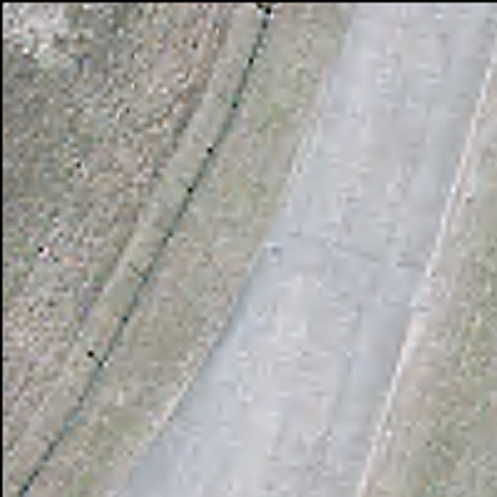
\includegraphics[width=\textwidth]{images/brewer_road_low.png}
%             \caption{"Low" quality road}
%             \label{fig:low_quality}
%         \end{subfigure}
%         \hfill
%         \begin{subfigure}{0.32\textwidth}
%             \centering
%             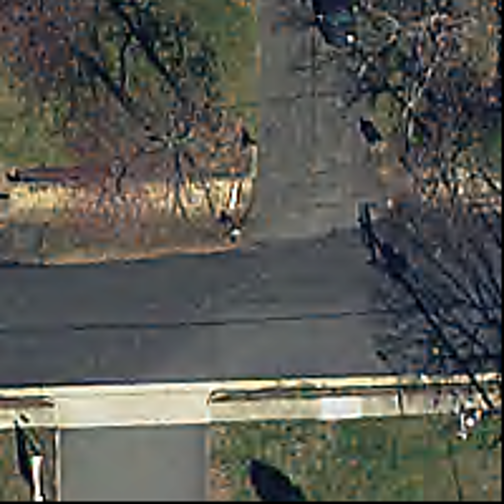
\includegraphics[width=\textwidth]{images/brewer_road_medium.png}
%             \caption{"Med" quality road}
%             \label{fig:medium_quality}
%         \end{subfigure}
%         \hfill
%         \begin{subfigure}{0.32\textwidth}
%             \centering
%             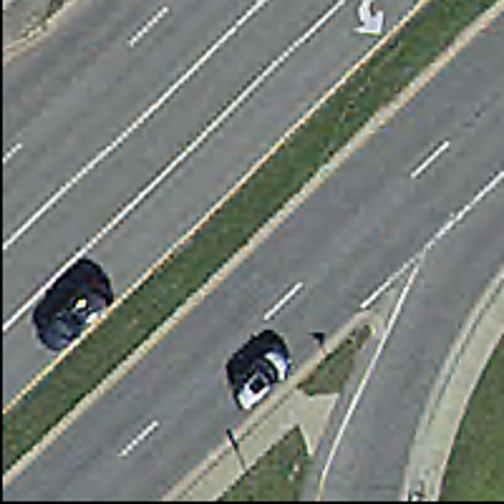
\includegraphics[width=\textwidth]{images/brewer_road_high.png}
%             \caption{"High" qualiy road}
%             \label{fig:high_quality}
%         \end{subfigure}
%         \caption{Examples: Satellite images of roads in Brewer et al. (2021)}
%         \label{fig:road_quality_egs}
%     \end{figure}
%     \begin{flushright}
%         \hyperlink{fine_tuning_workflow}{\beamergotobutton{Fine-tuning workflow}}
%     \end{flushright}        
% \end{frame}

\begin{frame}{Road Quality: Ohio satellite images}
    We use fine-tuned GPT 4O to predict the quality of Ohio Satellite Images collected from Google Earth.
    \begin{figure}[ht]
        \centering
        \begin{subfigure}{0.49\textwidth}
            \centering
            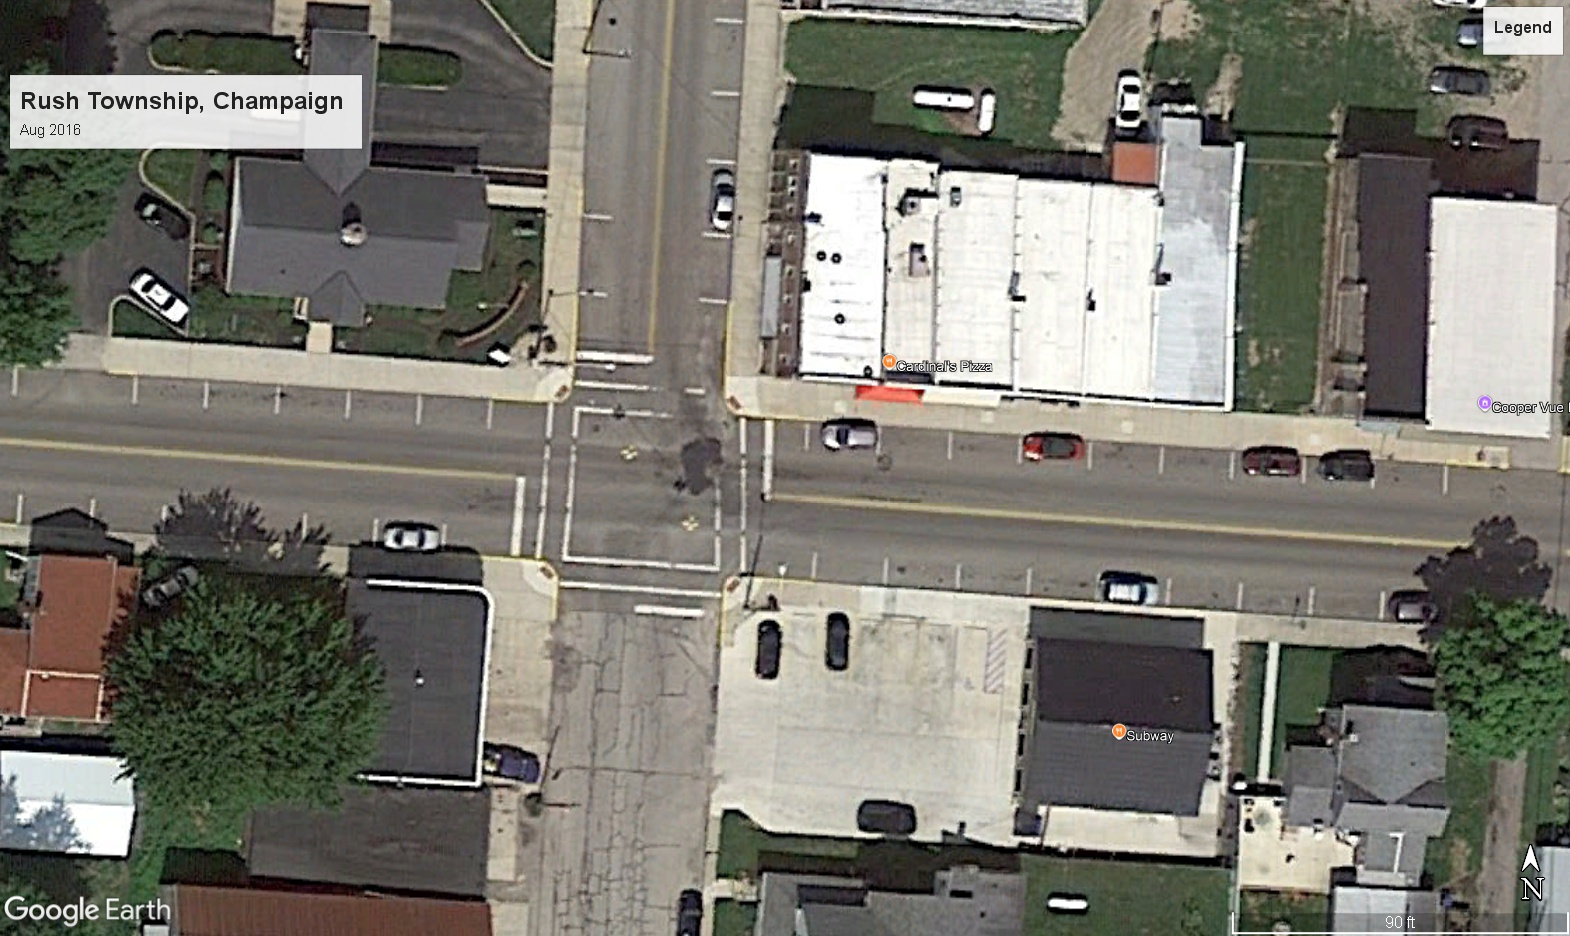
\includegraphics[width=\textwidth]{images/rush_twp_champaign_aug16.jpg}
            \caption{Road predicted as "Low" (0) quality}
            \label{fig:rush16}
        \end{subfigure}
        \hfill
        \begin{subfigure}{0.49\textwidth}
            \centering
            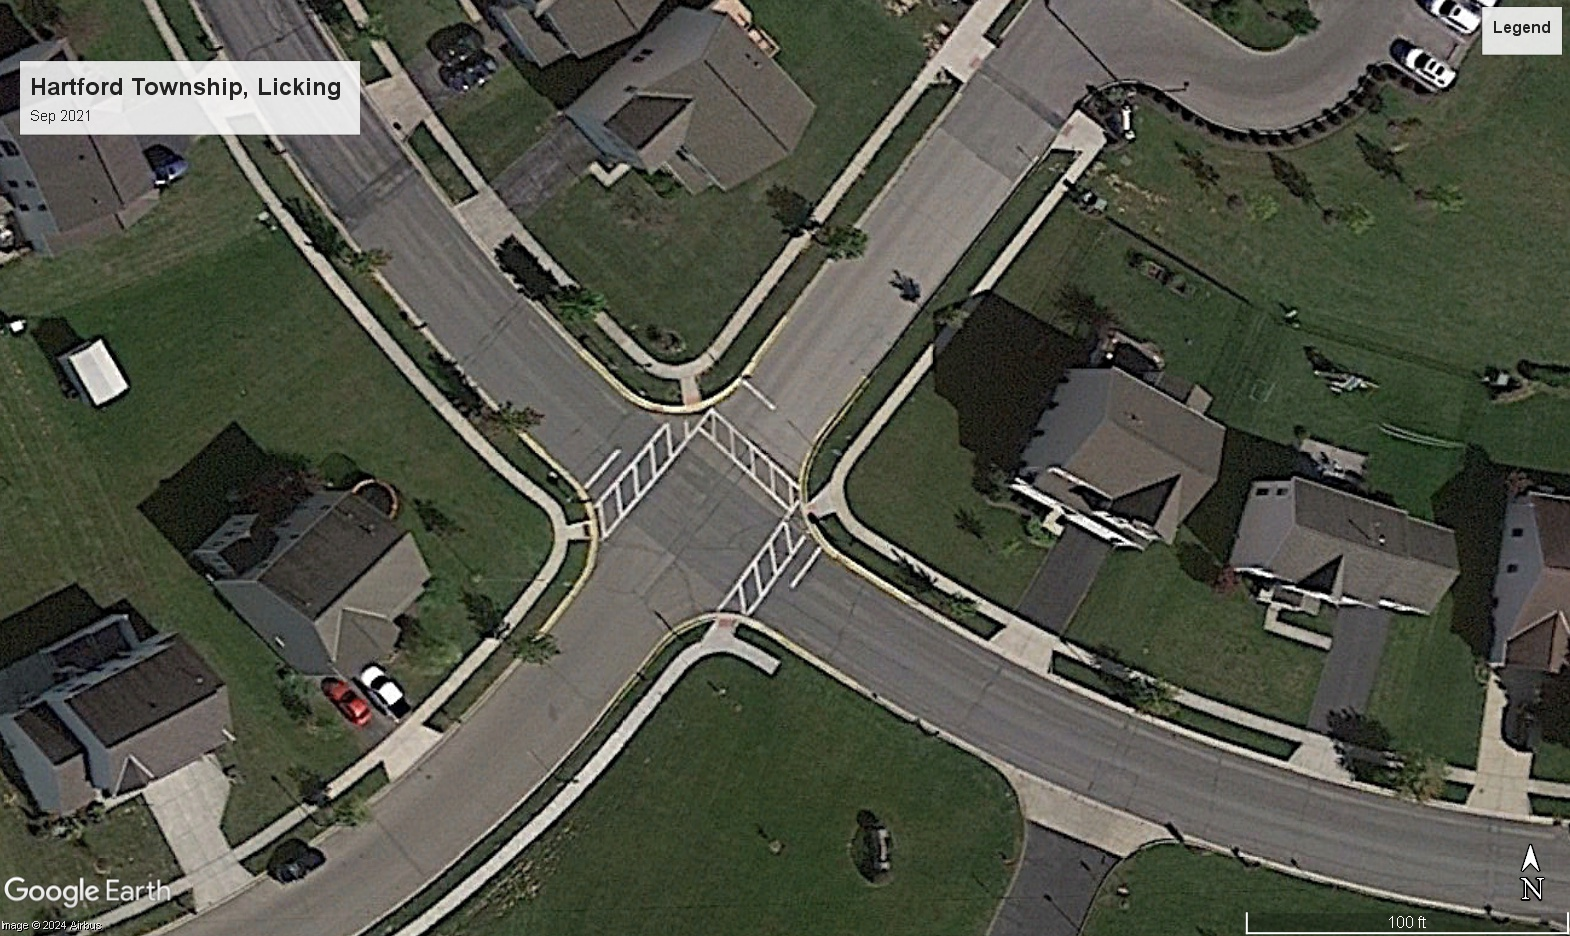
\includegraphics[width=\textwidth]{images/hartford_twp_licking_sep21.jpg}
            \caption{Road predicted as "High" (2) quality}
            \label{fig:hartford21}
        \end{subfigure}
        % \caption{Overall caption for the two images}
        \label{fig:ohio_satellite_images}
    \end{figure}

    Fine-tuned model results: Brewer’s metric of 70\%
\end{frame}

\begin{frame}{Road Quality: Ohio satellite images}
    We are interested in the {\bf change} in road quality before and after each election.
    \begin{figure}[ht]
        \centering
        \begin{subfigure}{0.49\textwidth}
            \centering
            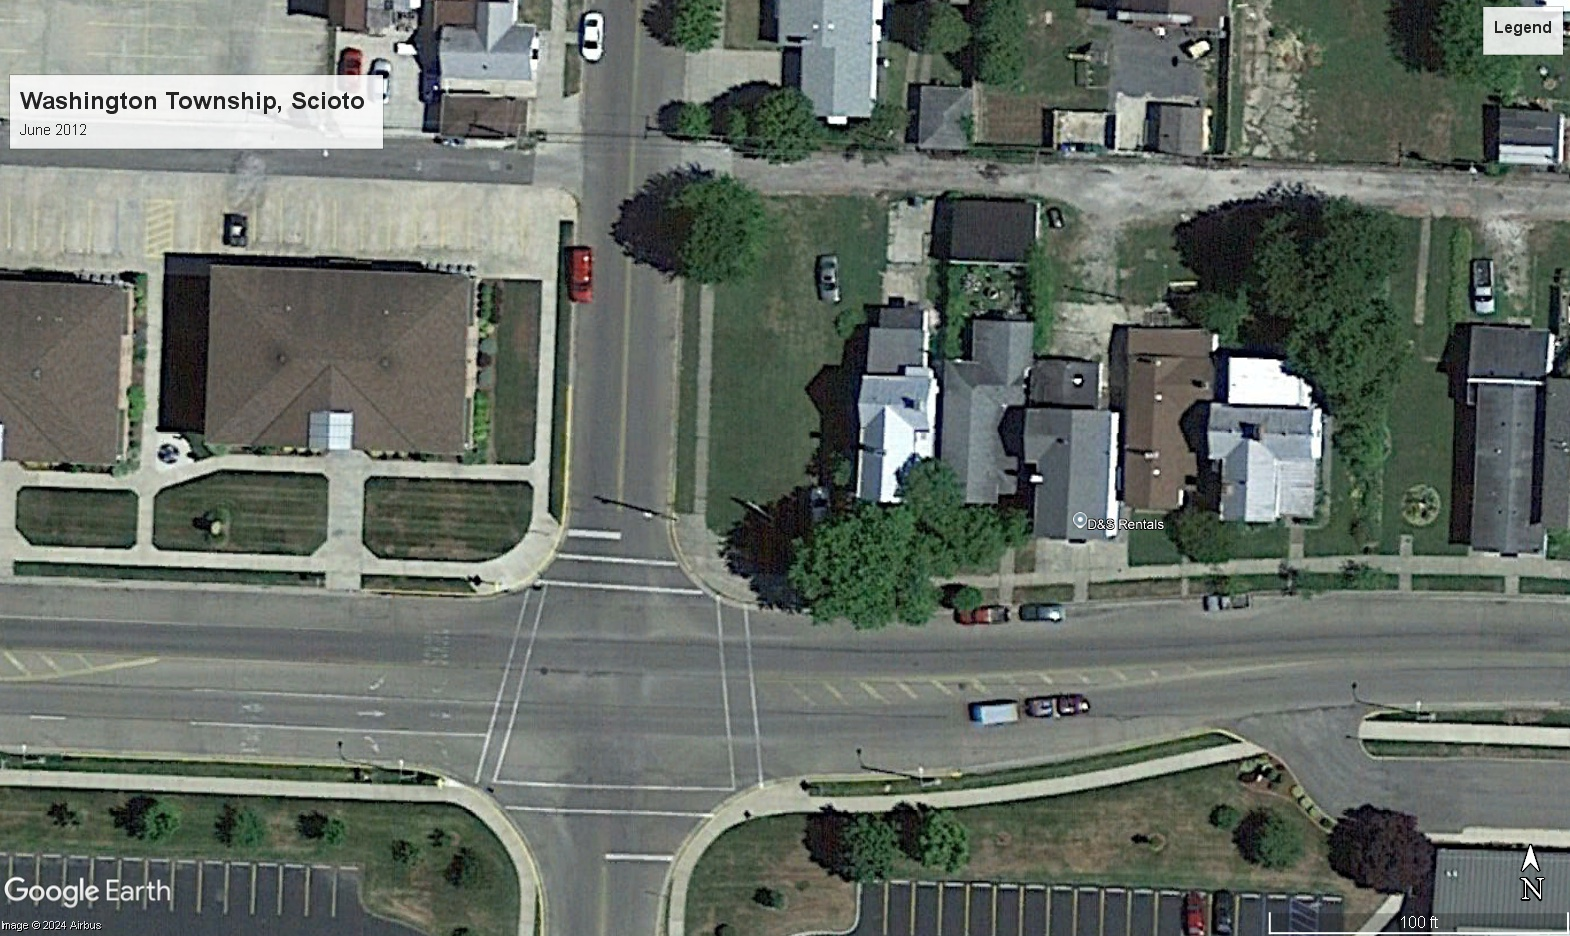
\includegraphics[width=\textwidth]{images/washington_twp_scioto_jun2012.jpg}
            \caption{Road predicted as "High" (2)}
            \label{fig:pred_2}
        \end{subfigure}
        \hfill
        \begin{subfigure}{0.49\textwidth}
            \centering
            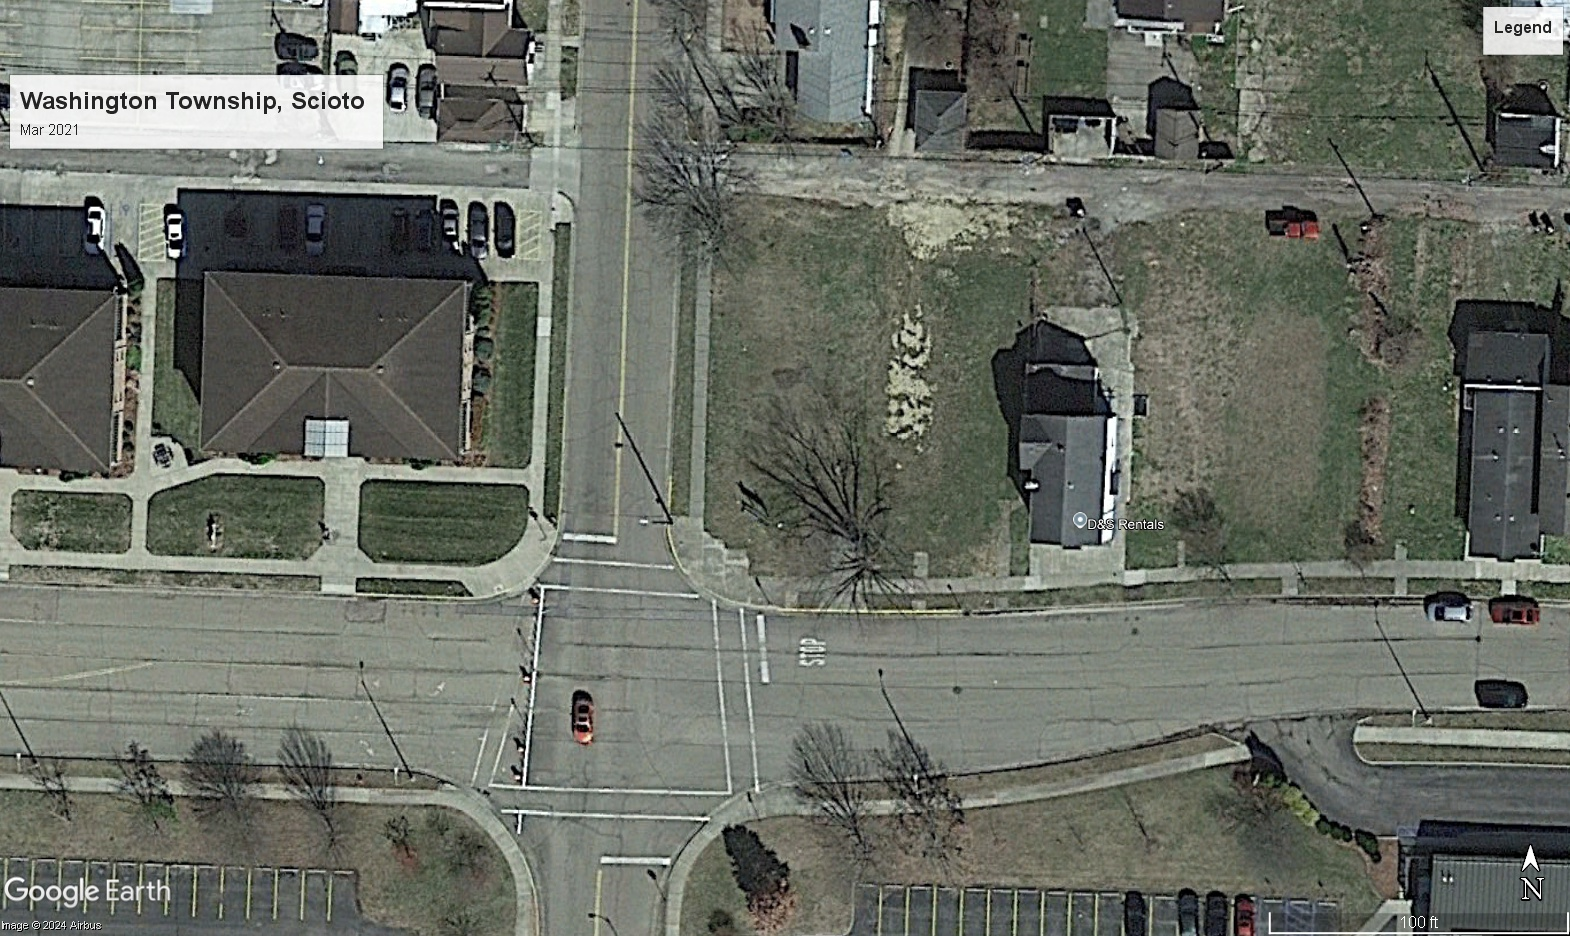
\includegraphics[width=\textwidth]{images/washington_twp_scioto_mar21.jpg}
            \caption{Road predicted as "Medium" (1)}
            \label{fig:pred_1}
        \end{subfigure}
        \caption{Washington Township, Scioto County, Ohio - 2012 vs. 2021}
        \label{fig:washington_pred}
    \end{figure}
\end{frame}

\begin{frame}{Predicted Road Quality: Before and After Election}
    \begin{table}
        \centering
        \caption{Predicted Road Quality by Treatment Status and Period}
        \label{tab:road_quality_panel}
        \resizebox{0.95\textwidth}{!}{
        \begin{tabular}{lcc}
        \toprule
        & \textbf{Treated (Failed Levy)} & \textbf{Control (Renewed Levy)} \\
        \midrule
        \multicolumn{3}{l}{\textbf{Panel A: Road Quality Rating (0, 1, 2)}} \\
        Pre-Election  & 1.38 & 1.00  \\
         & (0.770) & (0.913) \\
        Post-Election & 0.93 & 1.07 \\
         & (0.753) & (0.884) \\
        \addlinespace
        \multicolumn{3}{l}{\textbf{Panel B: Road Quality Score (1--100)}} \\
        Pre-Election  & 62.1 & 47.9 \\
         & (24.6) & (23.6) \\
        Post-Election & 50.5 & 52.1 \\
         & (29.3) & (28.4) \\
        \bottomrule
        \end{tabular}
        }
        % \vspace{0.2em}
        \scriptsize
        \textit{Notes:} Mean outcome per group, with standard deviations in parentheses. 
        % Treated = failed levy; Control = renewed levy.
    \end{table}
\end{frame}



\begin{frame}{Results: Road Quality Decline}
    \begin{table}[ht]
        \centering
        \caption{Effect of Road Maintenance Tax Levy Results on Road Quality}
        \label{tab:roadquality_estimates}
        \begin{threeparttable}
        \begin{tabular}{lcc}
        \hline\hline
        & \textbf{Cut Levies} & \textbf{Renewed Levies} \\
        \hline
        \multicolumn{3}{l}{\textbf{Panel A:}} \\
        Change in Road Quality Rating
         & -0.444\textsuperscript{**} & 0.067 \\[0.2cm]
         & (0.210) & (0.340) \\  
        \addlinespace[0.3em]
        \multicolumn{3}{l}{\textbf{Panel B:}} \\
        Change in Road Quality Score
         & -14.231\textsuperscript{**} & 1.585 \\[0.2cm]
         & (6.651) & (10.926) \\
        \hline
        \end{tabular}
        \begin{tablenotes}
        \small
        \item \textit{Notes:} Samples are set of referendums within the mean effective RD bandwidth from Table \ref{tab:median_sale_amount}. 
        \item Significance levels: 
    \textsuperscript{*}p $<$ 0.10,  
    \textsuperscript{**}p $<$ 0.05, 
    \textsuperscript{***}p $<$ 0.01.
        \end{tablenotes}
        \end{threeparttable}
    \end{table}
    {\bf This corresponds to 23-32\% deterioration in road quality.}    
\end{frame}



%-------------------------------------------------------
% Section 6: Results: House Prices
%-------------------------------------------------------
\section{House Prices}

\begin{frame}
    \begin{center}
        \vspace{2cm}
        {\LARGE \textbf{House Prices}}
    \end{center}
\end{frame}

\begin{frame}{Results: Discontinuity Graph}
    Median House Prices after 5 years: Control vs Treatment
    \begin{figure}[ht]
        \centering
        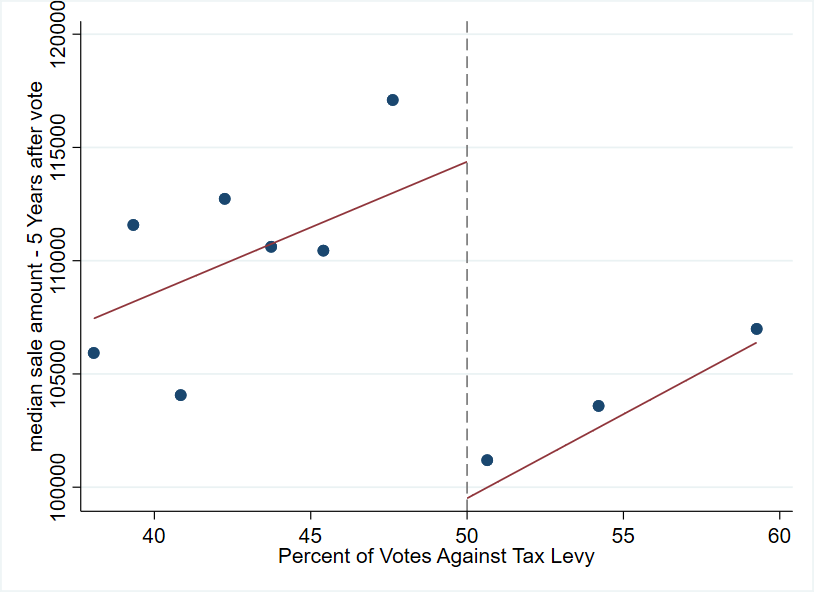
\includegraphics[width=0.8\textwidth]{images/rd_plot_year_5_after_vote.png}
        \caption{5 years {\bf after} the vote}
        \label{fig:house_prices_before_after}
    \end{figure}
\end{frame}

\begin{frame}[label=tes_gs_re]{Results: Effect of road tax cuts on House prices}
    \begin{figure}[ht]
        \centering
        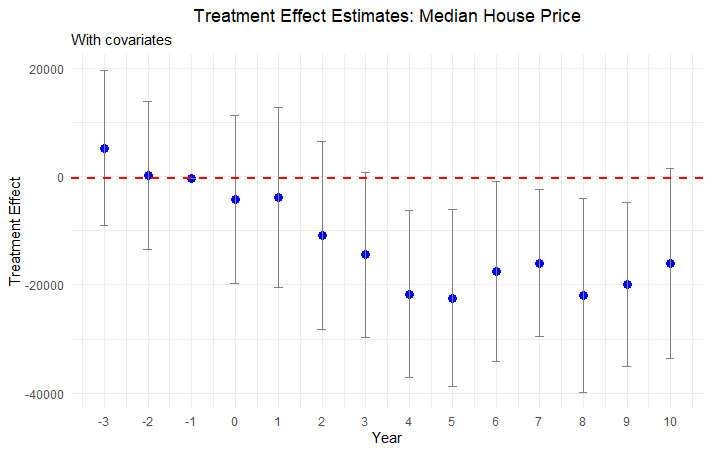
\includegraphics[width=0.75\textwidth]{images/tes_gs_reg.png}
        \caption{Year-by-year RD estimates}
        \label{fig:tes_gs_re}
    \end{figure}    
    {\bf \$15K or about 9\% over 10 years}
    \begin{flushright}
        \hyperlink{hp_estimates_tbl}{\beamergotobutton{Show Table of Estimates}}
    \end{flushright}
\end{frame}

\begin{frame}{Results: Urban vs. Rural}
    \begin{figure}[ht]
        \centering
        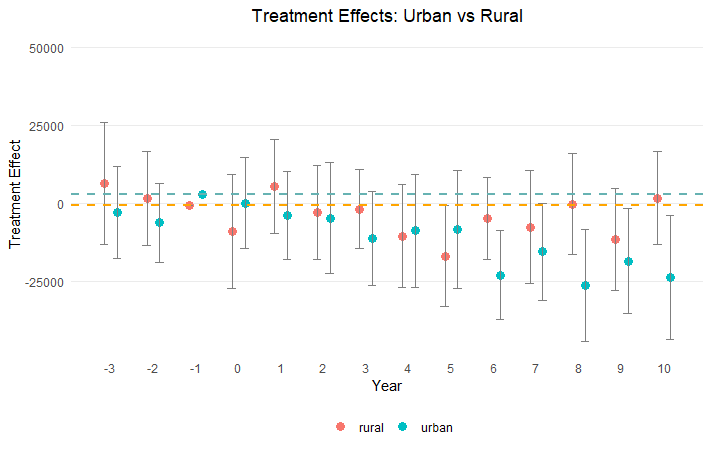
\includegraphics[width=0.85\textwidth]{images/tes_covs_ua_reg.png}
        \caption{Urban vs Rural}
        \label{fig:tes_covs_ua_reg}
    \end{figure}    
    {7.6\% of the home price over 10 years}
\end{frame}

\begin{frame}{Results: Dosage Response}
    \begin{figure}[ht]
        \centering
        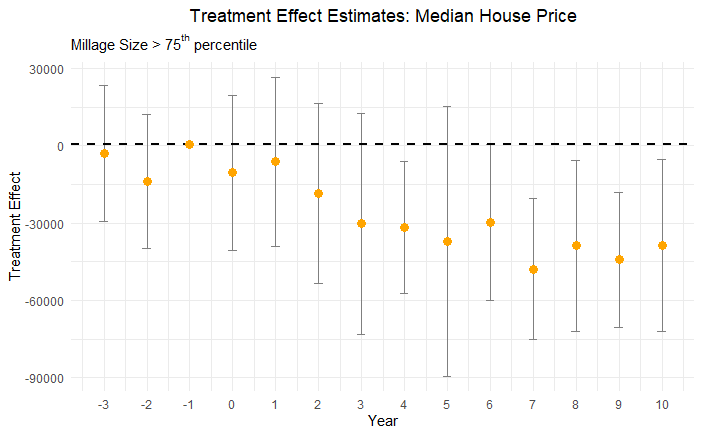
\includegraphics[width=0.85\textwidth]{images/tes_size_75.png}
        \caption{Highest quartile of tax cuts and house prices}
        \label{fig:tes_size_75}
    \end{figure}    
    {Larger tax cuts see a larger decline in house prices}
\end{frame}

\begin{frame}{Results: Expenses vs Cheaper Houses} 
    \begin{figure}[ht]
        \centering
        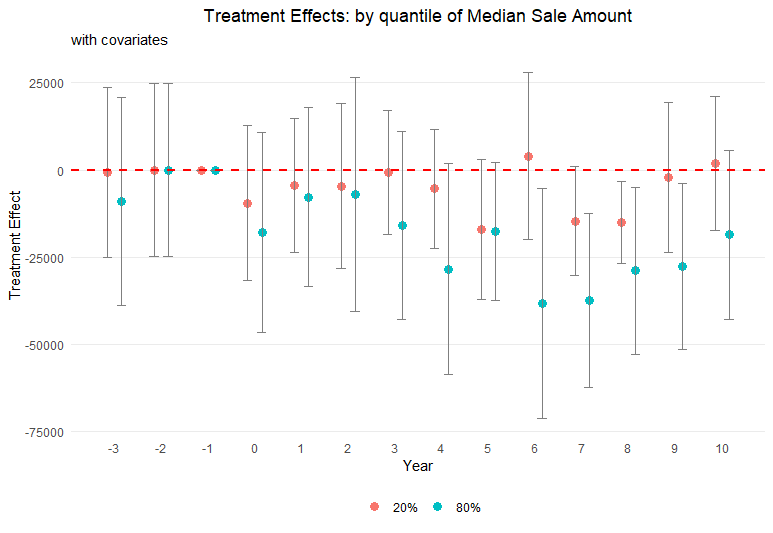
\includegraphics[width=0.85\textwidth]{images/tes_qte_re.png}
        \caption{Quantile Treatment Effects}
        \label{fig:tes_qte_re}
    \end{figure}    
\end{frame}

%-------------------------------------------------------
% Section 7: Conclusion
%-------------------------------------------------------
\section{Conclusion}

\begin{frame}{Conclusion}
    \begin{itemize}
        \item Expected Loss of 11\% in maintenance funds from failing to renew a road tax levy       
        \item \textbf{Cutting local road taxes} results in lower road quality (23\%) 
        \item Local road tax cuts decrease house prices by \$15K (9\%) 
        \begin{itemize}
            \item Urban areas and expensive houses experience more consistent declines than rural areas and cheaper houses
            \item Larger tax cuts lead to larger declines in house prices
        \end{itemize}
        \item \textbf{Trade-off:} Short-run tax relief is eclipsed by long-term private losses
        \item \textbf{Policy Implication:} Local tax decisions impact infrastructure maintenance and long-term property values
    \end{itemize}
\end{frame}

% Thank you slide
\begin{frame}{Thank You}
    \begin{center}
        % \Large{Thank you for your attention!}\\
        \Large{Scan for full paper:}  
        \vskip 0.2cm
        
\includegraphics[width=0.35\textwidth]{images/QR.png}
    \end{center}
\end{frame}

%------------------------------------------------------- 
% Appendix
%-------------------------------------------------------
\appendix
\section{Appendix}


\begin{frame}[label=gdp_and_roads]{Roads and GDP}
    \begin{figure}[ht]
        \centering
        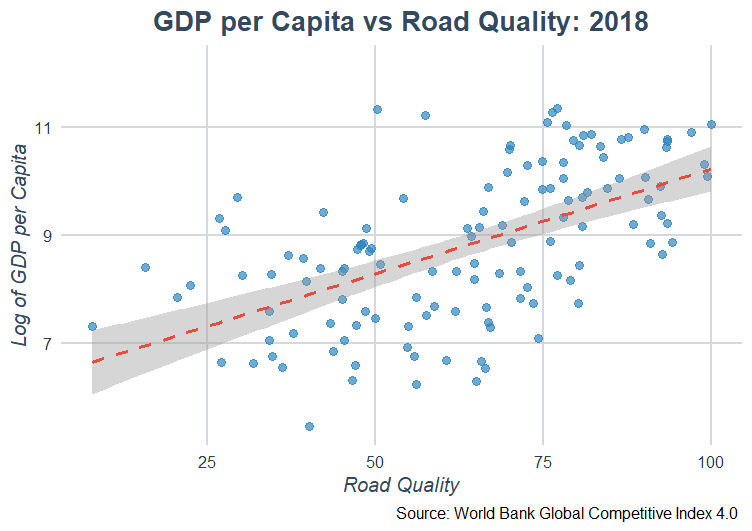
\includegraphics[width=0.8\textwidth]{images/road_quality_vs_gdp_per_cap.png}
        % \caption{Impact of Road Quality on GDP Growth}
        \label{fig:roads_gdp}
    \end{figure}
    \begin{flushright}
        \hyperlink{motivation}{\beamergotobutton{Main}}
    \end{flushright}       
\end{frame}

\begin{frame}[label=odot_who_does_what]{Background}
    Who funds the roads in Ohio?
    \begin{figure}[ht]
        \centering
        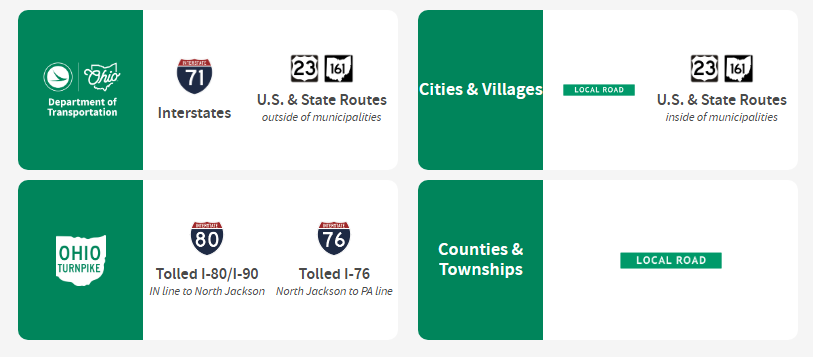
\includegraphics[width=0.9\textwidth]{images/odot_who_does_what.png}
        \caption{Source: Ohio Department of Transportation}
        \label{fig:odot_who_does_what}
    \end{figure}
    \begin{flushright}
        \hyperlink{who_funds_roads}{\beamergotobutton{back to main}}
    \end{flushright}
\end{frame}

\begin{frame}{Background}
    ODOT Disbursement of Funds
    \begin{figure}[ht]
        \centering
        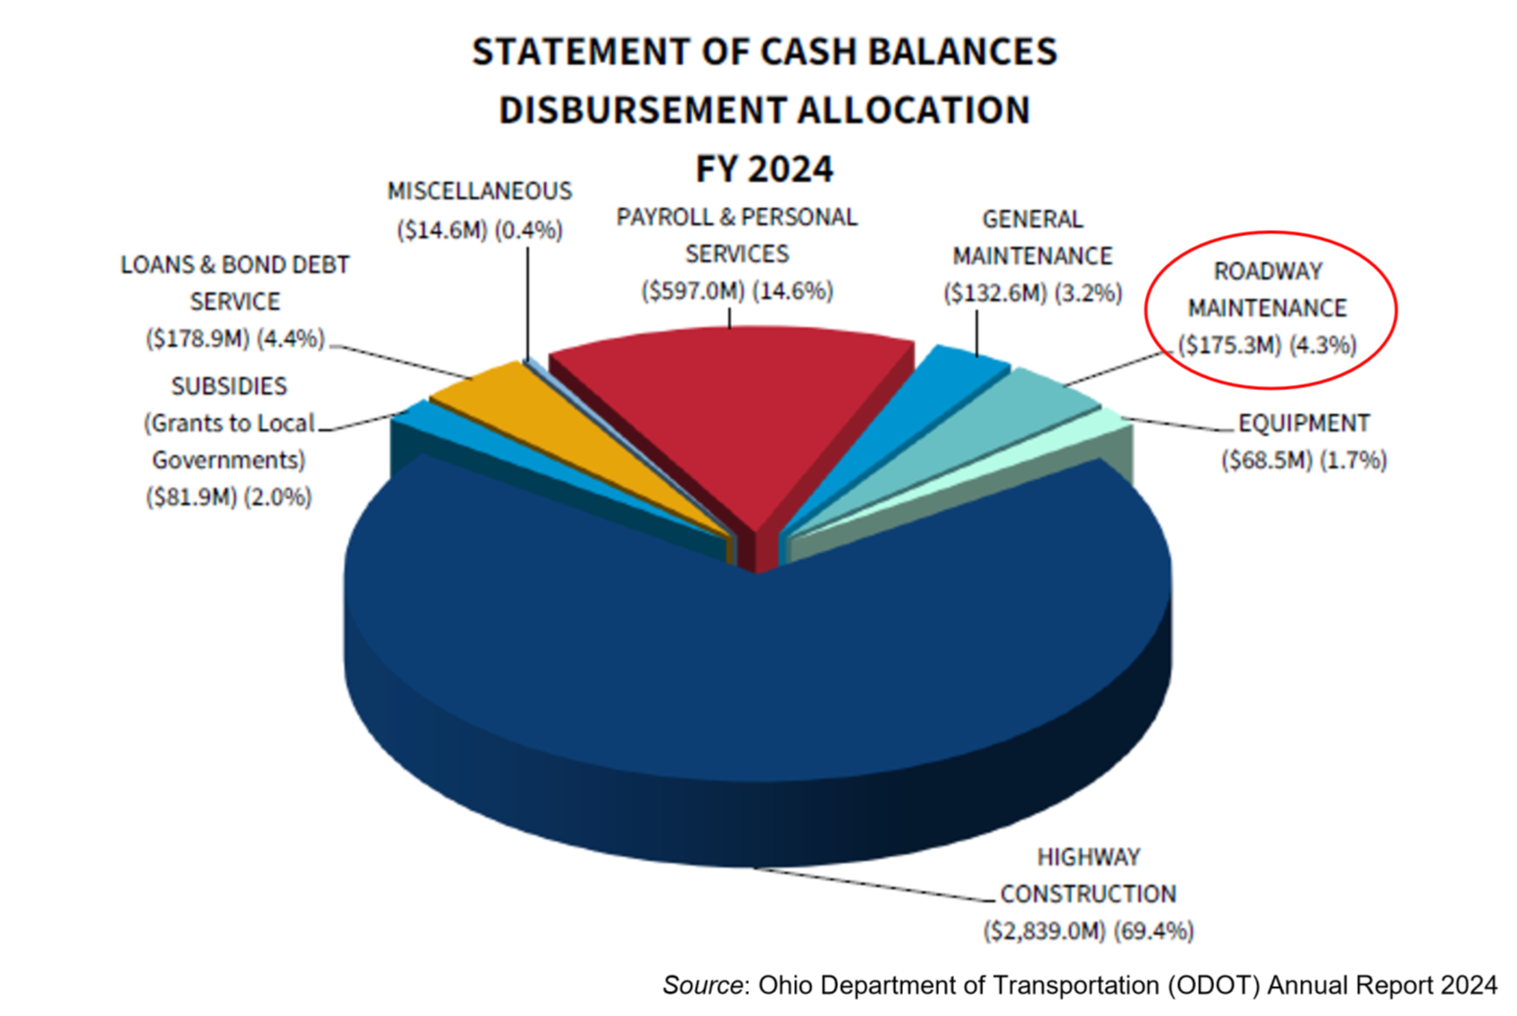
\includegraphics[width=0.9\textwidth]{images/odot_2024.png}
        \caption{Source: Ohio Department of Transportation}
        \label{fig:odot_2024}
    \end{figure}
    \begin{flushright}
        \hyperlink{who_funds_roads}{\beamergotobutton{back to main}}
    \end{flushright}
\end{frame}

% References
% \begin{frame}[allowframebreaks]{References}
%     \bibliographystyle{apalike}

% \end{frame}

\begin{frame}{Ohio Auditor of State Reports}
    \begin{figure}[ht]
        \centering
        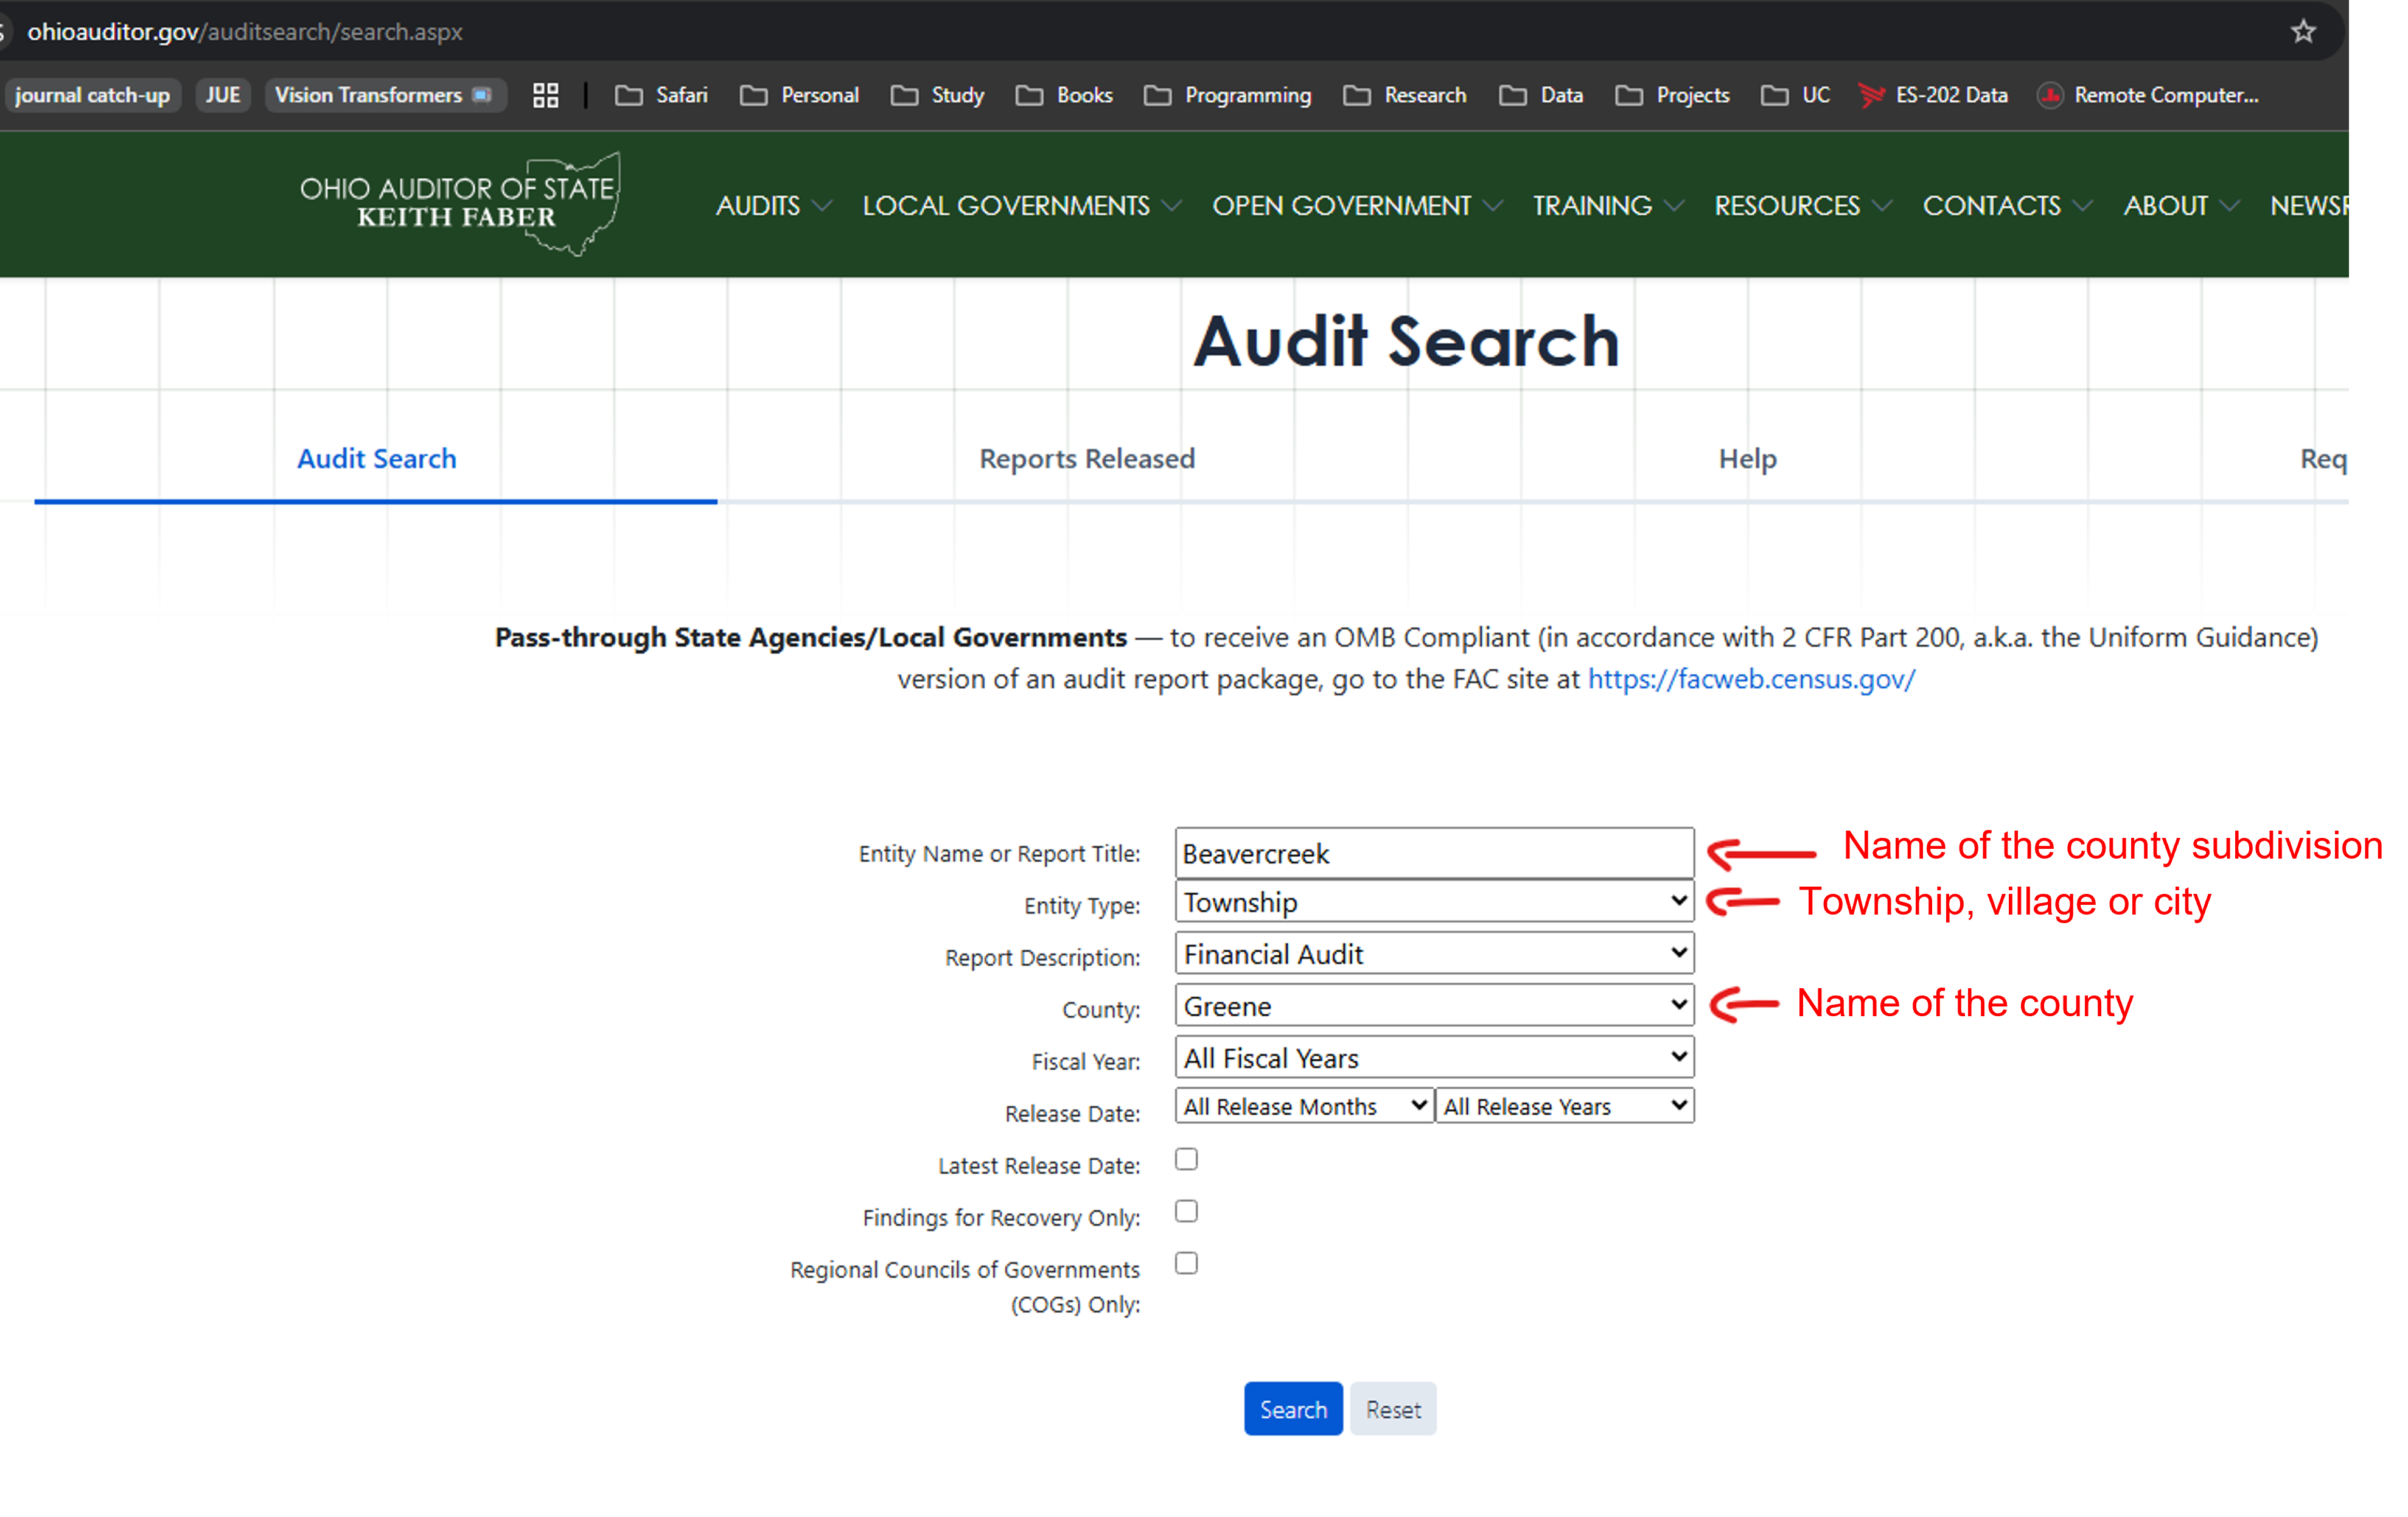
\includegraphics[width=1.0\textwidth]{images/ohio_auditor_of_state_reports_1.png}
        \caption{Ohio Auditor of State Reports Collection}
        \label{fig:auditor_reports1}
    \end{figure}
\end{frame}

\begin{frame}{Ohio Auditor of State Reports}
    \begin{figure}[ht]
        \centering
        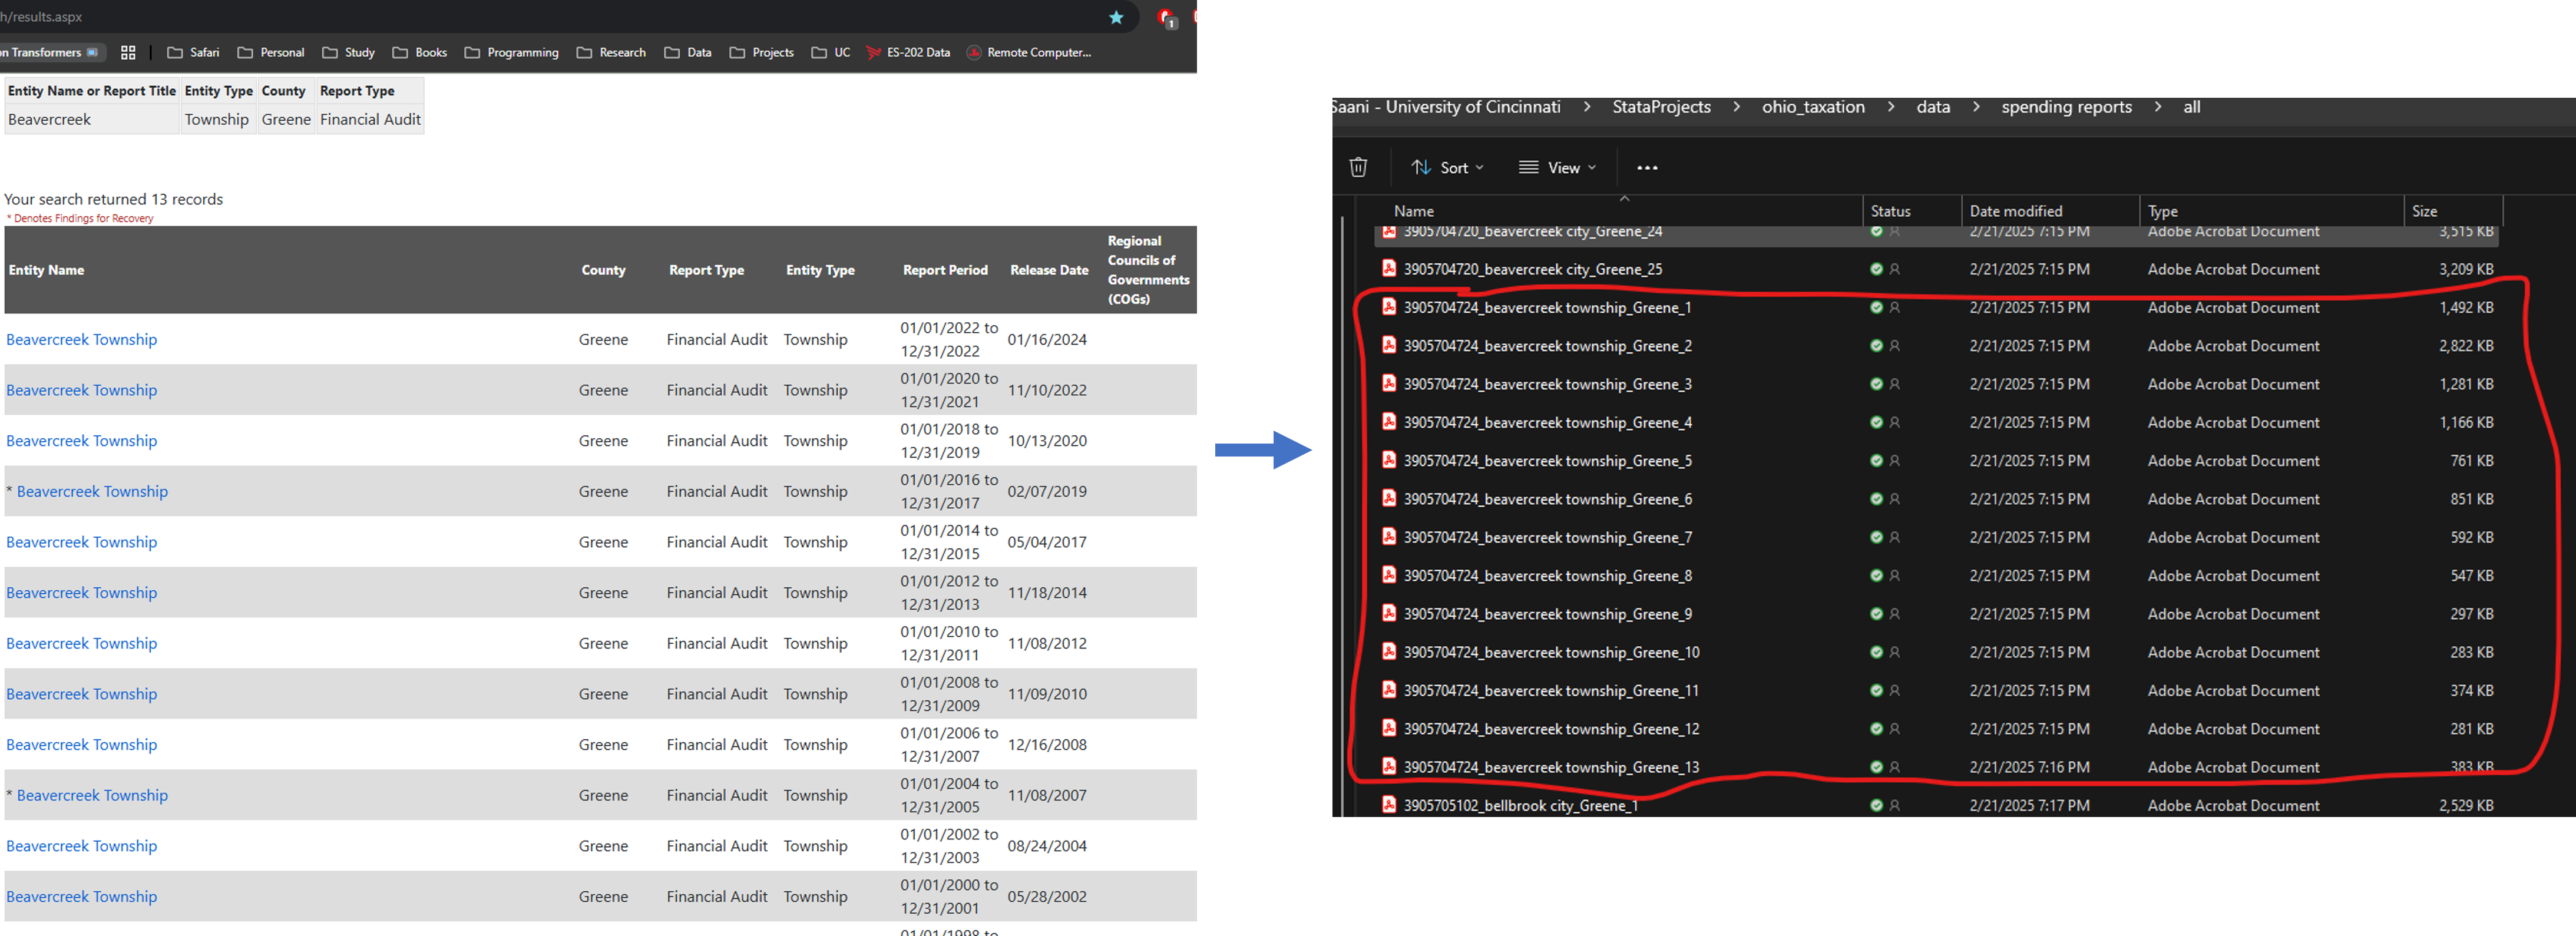
\includegraphics[width=1.0\textwidth]{images/ohio_auditor_of_state_reports_2.png}
        \caption{Ohio Auditor of State Reports Collection}
        \label{fig:auditor_reports2}
    \end{figure}
\end{frame}

\begin{frame}{Covariate Balance Table}
    \begin{figure}[ht]
        \centering
        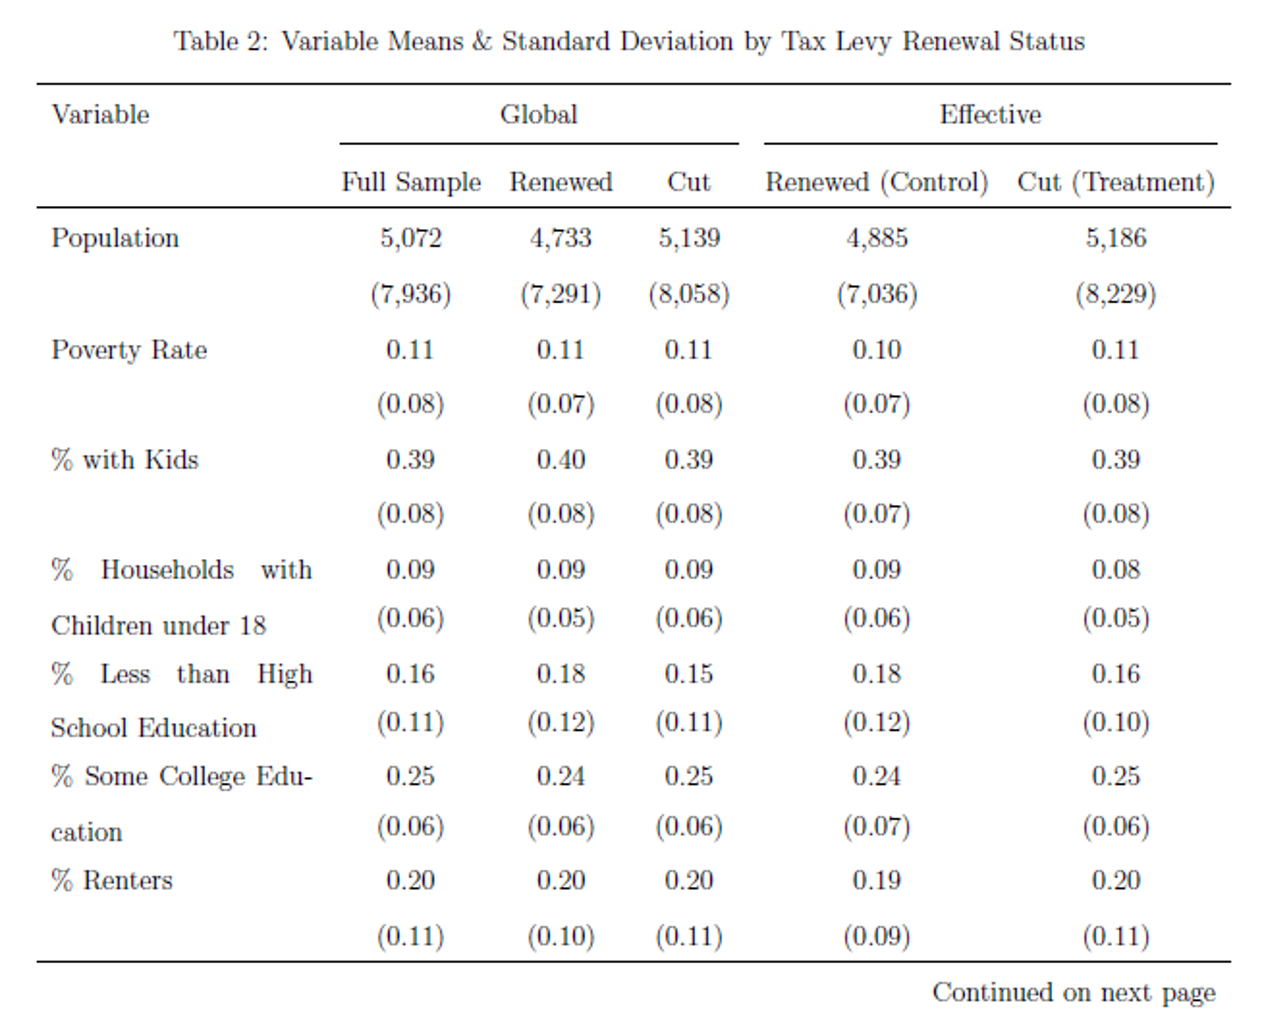
\includegraphics[width=0.9\textwidth]{images/cov_bal_table_1.png}
        \label{fig:covariate_balance_table1}
    \end{figure}
\end{frame}

\begin{frame}{Covariate Balance Table}
    \begin{figure}[ht]
        \centering
        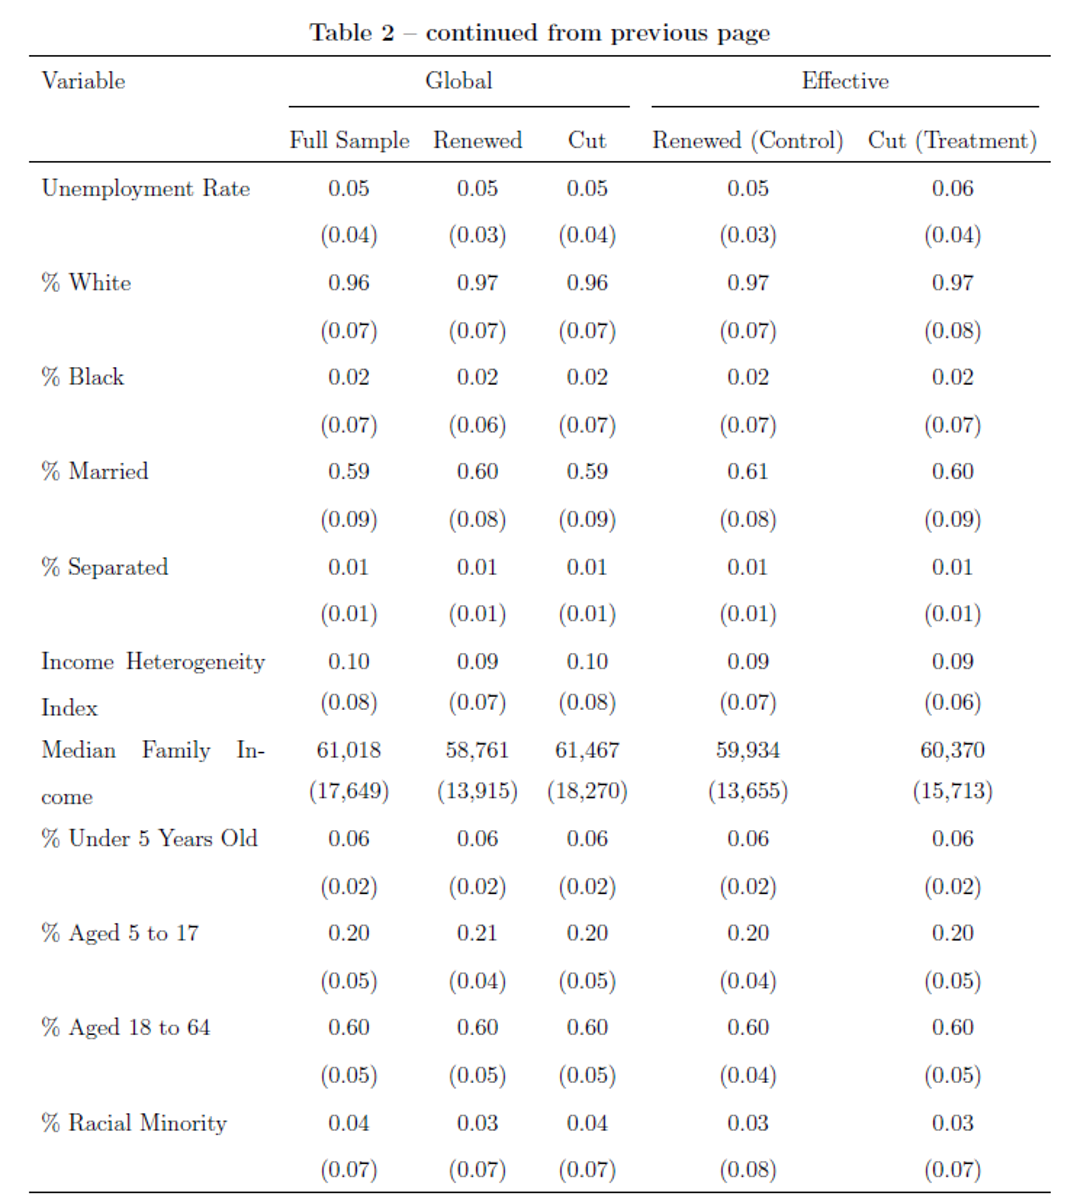
\includegraphics[width=0.65\textwidth]{images/cov_bal_table_2.png}
        \label{fig:covariate_balance_table2}
    \end{figure}
\end{frame}

\begin{frame}{No ``bunching''. Fair elections.}
    \begin{figure}[ht]
        \centering
        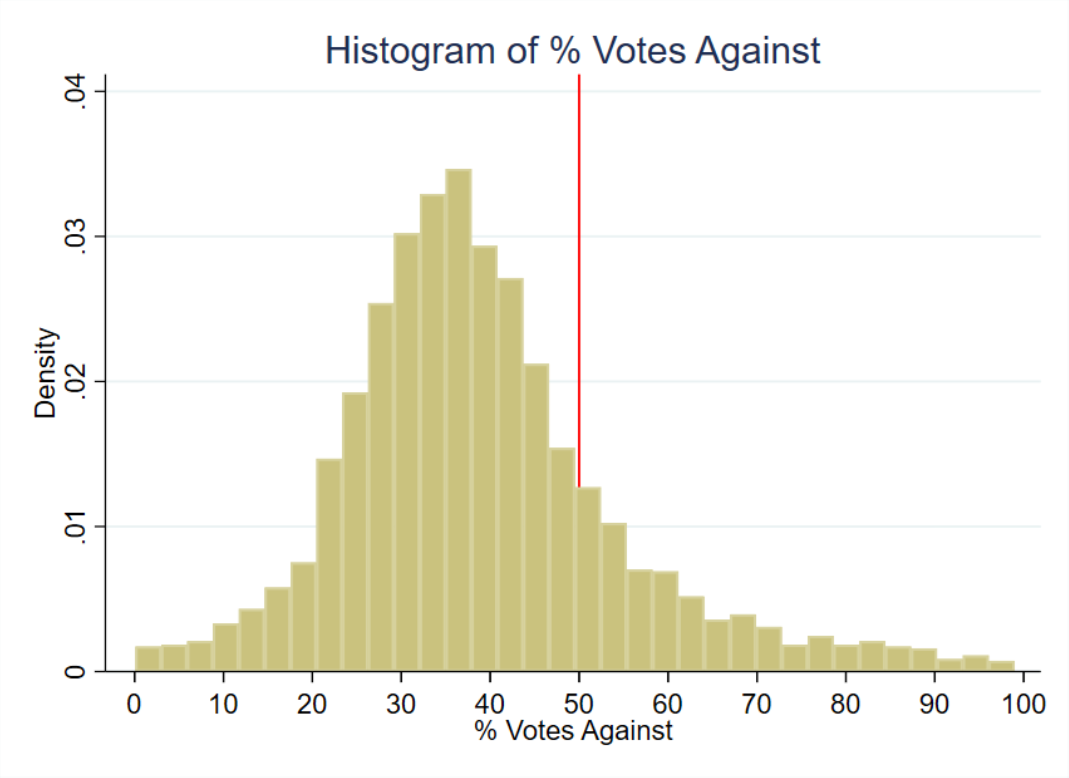
\includegraphics[width=0.8\textwidth]{images/pct_votes_against_histogram.png}
    \end{figure}
\end{frame}

\begin{frame}[label=spending_measure_2]{Spending measures: Metric 2 work-in-progress}
    \begin{itemize}
        \item We scraped Ohio Auditor of State website to collect all available financial reports for townships, cities and villages. This gives us over 10,000 reports.
        \item Reports contain taxes collected and expenditures incurred by the local government, for various purposes. 
        \item  We will check the immediate or eventual changes in funding after a tax cut.
    \end{itemize}        
    \begin{flushright}
        \hyperlink{spending_measures}{\beamergotobutton{Back to Spending Measures}}
    \end{flushright}      
\end{frame}

\begin{frame}[label=fine_tuning_workflow]{Road Quality: fine-tuning workflow}
    \begin{figure}[ht]
        \centering
        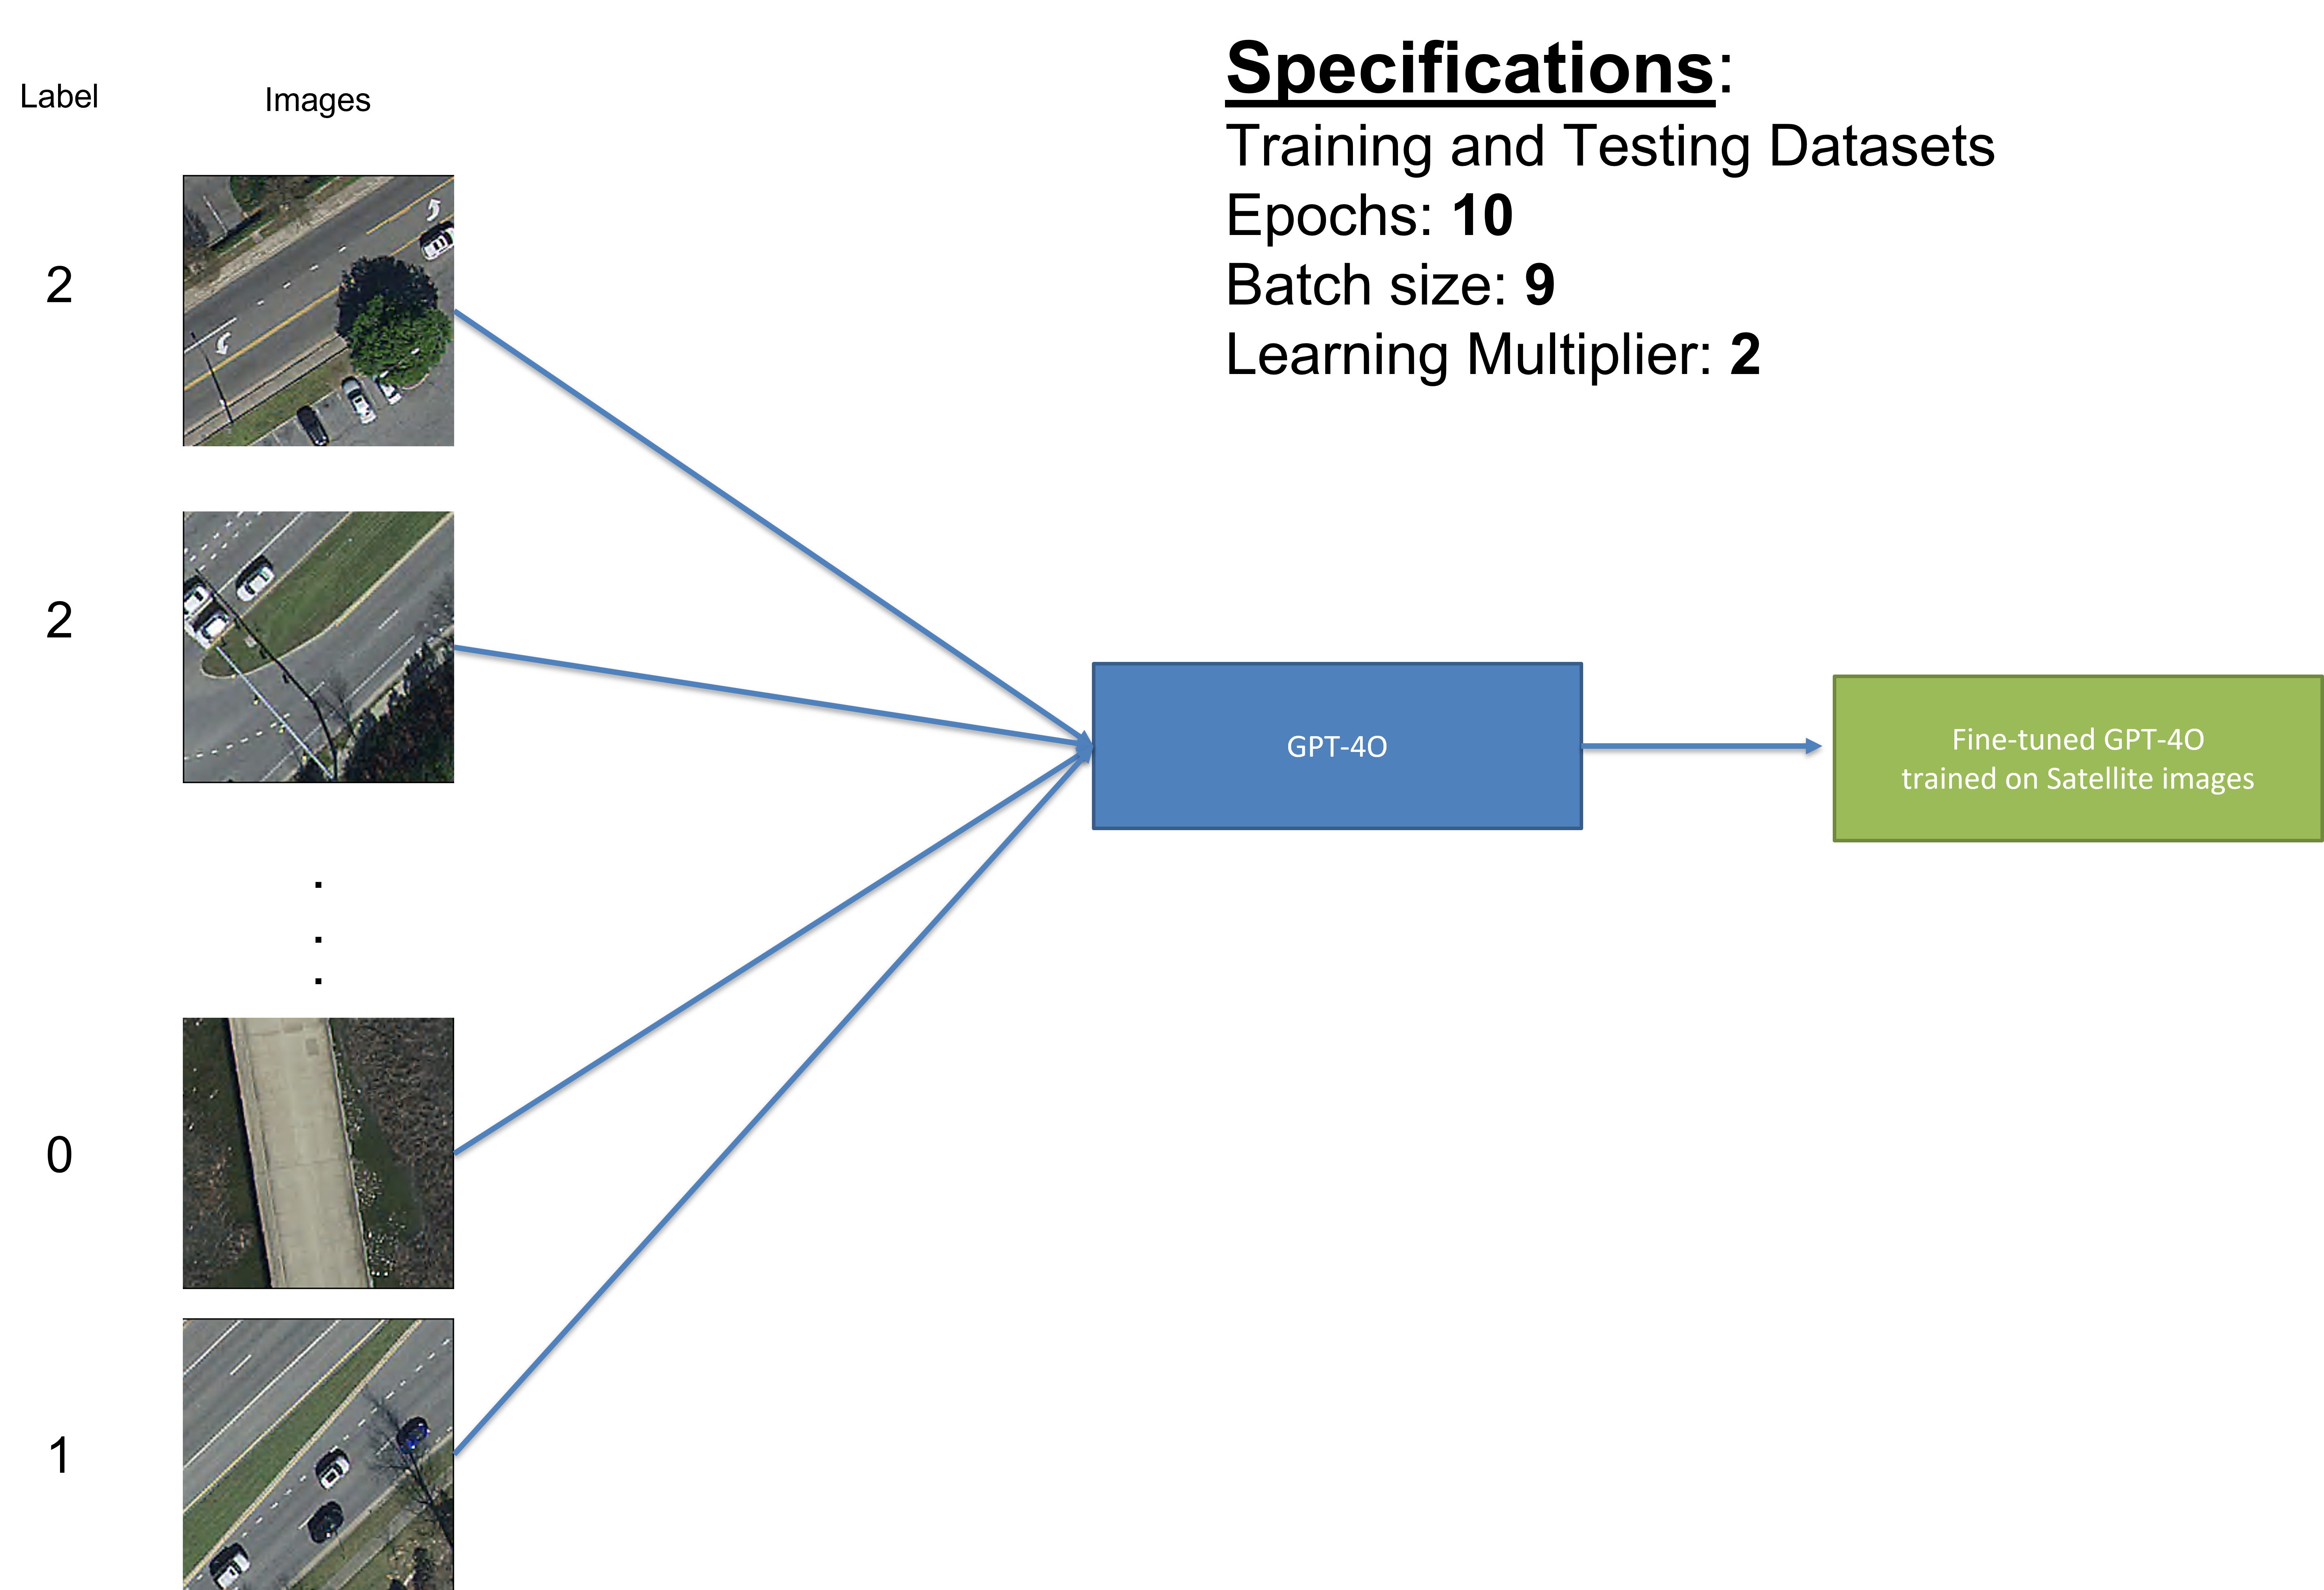
\includegraphics[width=0.9\textwidth]{images/fine_tuning_workflow.png}
        \caption{Fine-tuning workflow for road quality classification}        
        \label{fig:road_quality_workflow}
    \end{figure}
    \begin{flushright}
        \hyperlink{brewer_training}{\beamergotobutton{Brewer's training data}}
    \end{flushright}
\end{frame}

\begin{frame}[label=streetview]{Road quality, Method 2: Streetview images}
    \begin{center}
        Kaya, Yasin (2024): Road damage labeled Streetview data from 6 different countries.
        \begin{figure}[ht]
            \centering
            \begin{subfigure}{0.49\textwidth}
                \centering
                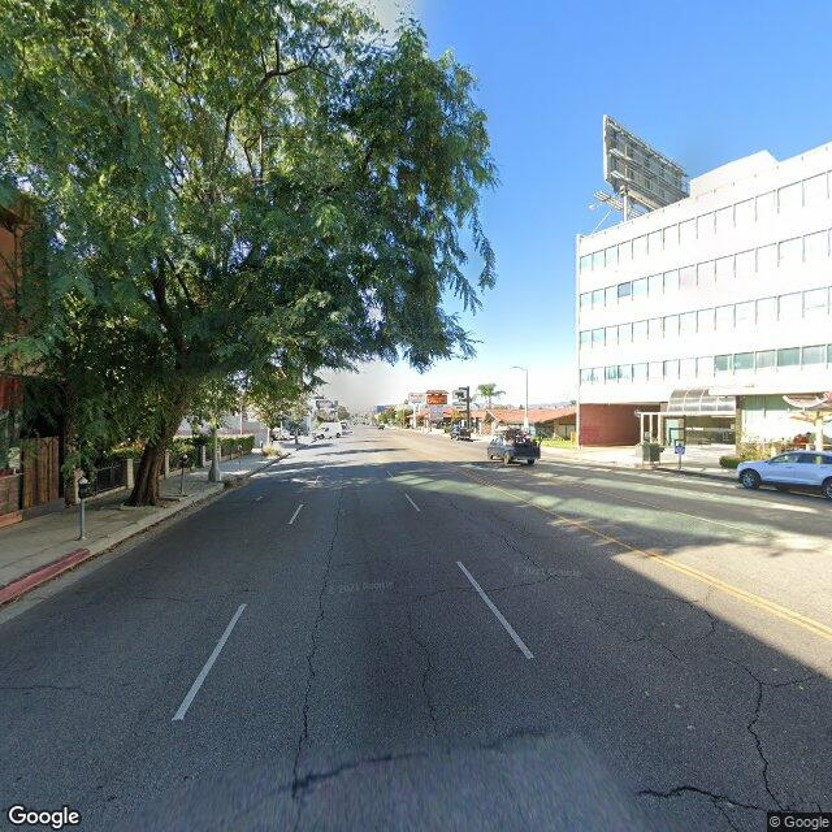
\includegraphics[width=\textwidth]{images/streetview_training_data_example.jpg}
                \caption{000122}
                \label{fig:streetview_image1}
            \end{subfigure}
            \hfill
            \begin{subfigure}{0.49\textwidth}
                \centering
                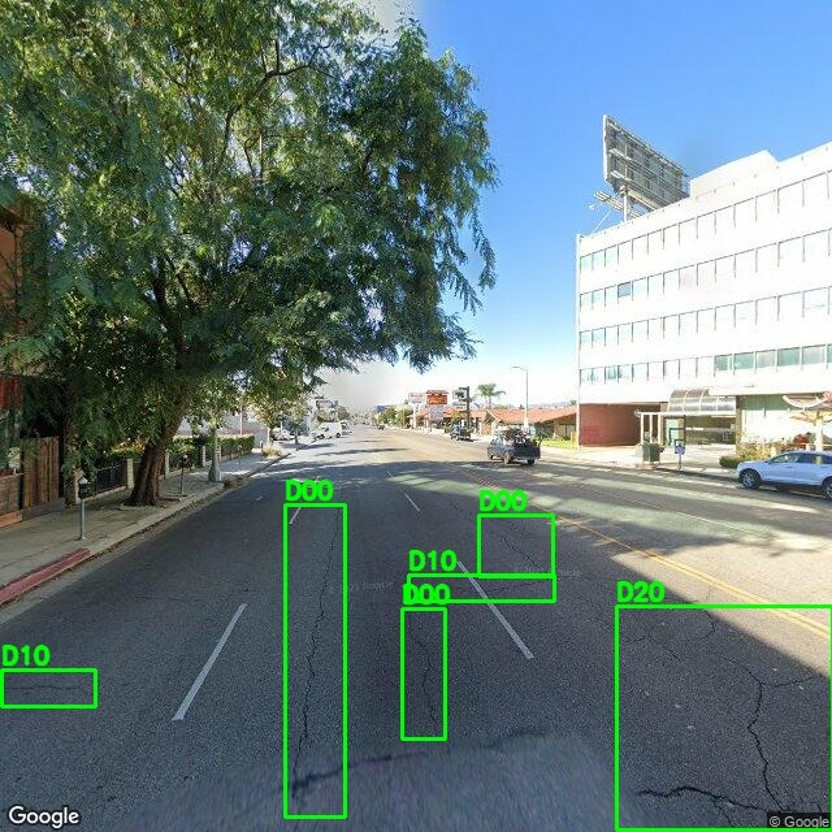
\includegraphics[width=\textwidth]{images/streetview_training_data_example_labeled.jpg}
                \caption{000122 - labeled}
                \label{fig:streetview_image2}
            \end{subfigure}
            % \caption{Overall caption for the two images}
            % \label{fig:side_by_side_images}
        \end{figure}
    \end{center}
    \begin{flushright}
        \hyperlink{road_quality_measures}{\beamergotobutton{Road Quality Measures}}
    \end{flushright}
\end{frame}

\begin{frame}{Road quality, Method 2: Streetview images}
    \begin{center}
        Using Google Streetview API, we collect Streetview images before and after an election in a subdivision.
        \begin{figure}[ht]
            \centering
            \begin{subfigure}{0.49\textwidth}
                \centering
                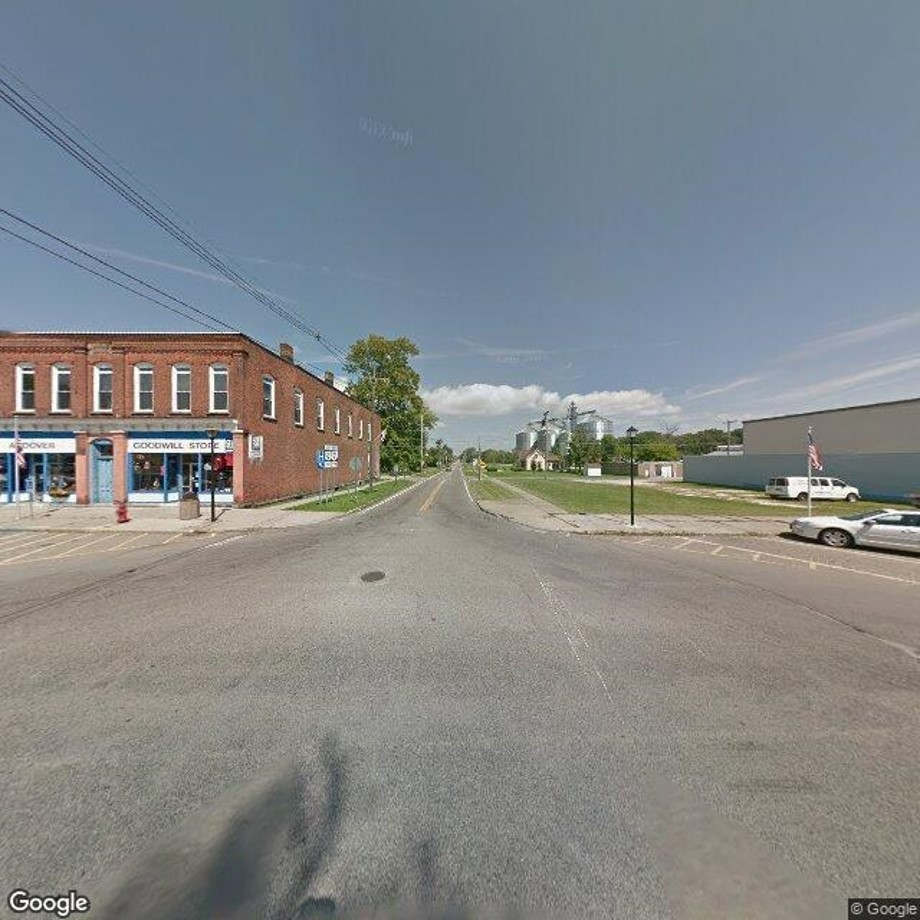
\includegraphics[width=\textwidth]{images/streetview_api_road_before.jpg}
                \caption{Before the election}
                \label{fig:streetview_1}
            \end{subfigure}
            \hfill
            \begin{subfigure}{0.49\textwidth}
                \centering
                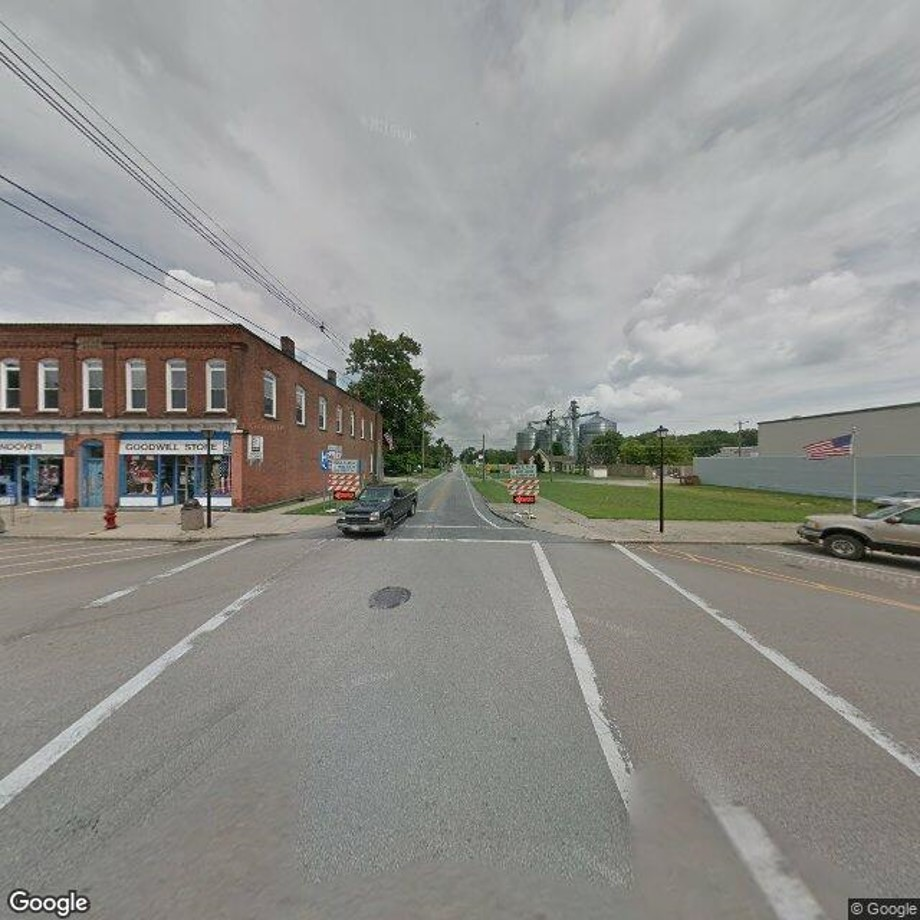
\includegraphics[width=\textwidth]{images/streetview_api_road_after.jpg}
                \caption{After the election}
                \label{fig:streetview_22}
            \end{subfigure}
        \end{figure}
    \end{center}
\end{frame}

\begin{frame}[label=rqs]{Road Quality Score (RQS): Continuous Metric}
    \begin{itemize}
        \item \textbf{Why RQS?} Converts model's discrete road quality rating into a continuous 1--100 scale, similar to ODOT's Pavement Condition Rating.
        \item \textbf{How?} Combines predicted rating ($\hat{r}$) and model confidence ($\hat{c}$) using:
        \begin{equation*}
            \text{RQS} = 1 + [
            (\hat{r} + \tau \cdot \hat{c}) \cdot w \cdot \mathbb{I}\{\hat{r} \ne 0\}
            + (1 - \tau) \cdot \hat{c} \cdot w  \cdot \mathbb{I}\{\hat{r} = 0\} ]
        \end{equation*}
        \item \textbf{Interpretation:} RQS ranges from 1 (poor) to 100 (high) quality.
        \item \textbf{Use:} Enables comparison with ODOT's Pavement Condition Rating (PCR) and other continuous metrics.
    \end{itemize}
    \begin{flushright}
        \hyperlink{road_quality_measures}{\beamergotobutton{Back to Main}}
    \end{flushright}
\end{frame}

\begin{frame}[label=hp_estimates_tbl]{Results: Effect of road tax cuts on House prices}
    \begin{table}[ht]
    \centering
    \caption{\scriptsize Effect on median house prices of failing to renew a road tax levy}
    \label{tab:median_sale_amount}
    \resizebox{\textwidth}{!}{%
    \begin{tabular}{p{2.5cm}ccccccc}
    \hline
    \scriptsize Year relative to vote & \scriptsize $t + 4$ & \scriptsize $t + 5$ & \scriptsize $t + 6$ & \scriptsize $t + 7$ & \scriptsize $t + 8$ & \scriptsize $t + 9$ & \scriptsize $t + 10$ \\
    \hline
    \scriptsize Treatment effect & \scriptsize -21,638 & \scriptsize -22,271 & \scriptsize -17,336 & \scriptsize -15,975 & \scriptsize -21,993 & \scriptsize -19,857 & \scriptsize -16,090 \\
    \scriptsize Standard error   & \scriptsize (7,731) & \scriptsize (8,864) & \scriptsize (8,331) & \scriptsize (7,248) & \scriptsize (9,079) & \scriptsize (7,751) & \scriptsize (9,027) \\
    \scriptsize Effective bandwidth ($h$) & \scriptsize 8.540 & \scriptsize 10.796 & \scriptsize 9.840 & \scriptsize 13.158 & \scriptsize 8.246 & \scriptsize 7.285 & \scriptsize 6.241 \\
    \scriptsize Bias bandwidth ($b$) & \scriptsize 16.379 & \scriptsize 19.879 & \scriptsize 17.397 & \scriptsize 23.413 & \scriptsize 15.255 & \scriptsize 14.091 & \scriptsize 16.266 \\
    \scriptsize Effective Observations & \scriptsize 688 & \scriptsize 883 & \scriptsize 769 & \scriptsize 1,061 & \scriptsize 591 & \scriptsize 505 & \scriptsize 402 \\
    \scriptsize Total Observations & \scriptsize 2,614 & \scriptsize 2,531 & \scriptsize 2,438 & \scriptsize 2,324 & \scriptsize 2,199 & \scriptsize 2,115 & \scriptsize 2,017 \\
    \hline
    \end{tabular}%
    }
    \vspace{-0.2cm}
    \begin{tablenotes}
    \scriptsize
    \item \textit{Notes:} Outcome is median house price in constant 2010 U.S. dollars. Unit of observation is the city-year. Treatment effects for years prior to $t + 4$ are statistically insignificant at the 5\% level. The regressions include covariates related to the demographics and socioeconomic factors of the cities, drawn from covariates table.
    \end{tablenotes}
    \end{table}
    \begin{flushright}
        \hyperlink{tes_gs_re}{\beamergotobutton{Back to Results Figure}}
    \end{flushright}
\end{frame}

\begin{frame}{Robustness Checks}
    \begin{table}[ht!]
        \centering
        \caption{Correlation of Road Tax Levy Referenda Results with Other Types of Levies}
        \begin{tabular}{lcccccc}
        \toprule
        & Police & Fire & Recreational & School \\
        \midrule
        Estimate & 0.248 & 0.053 & 0.015 & -0.024 \\
        & (0.153) & (0.043) & (0.317) & (0.092) \\
        \bottomrule
        \end{tabular}
        \begin{minipage}{\textwidth}
        \footnotesize
        \textit{Notes:} This table presents coefficients from regressions correlating road tax levy referendum outcomes with outcomes for other types of levies (police, fire, recreational, school). Standard errors are reported in parentheses. All regression control for year and neighborhood fixed effects, as well as neighborhood characteristics. The school levy analysis is conducted at the county level, while all other analyses are at the county subdivisions level. Statistical significance levels are indicated as follows: *** $p<0.01$, ** $p<0.05$, * $p<0.1$.
        \end{minipage}
    \end{table}
\end{frame}

\begin{frame}[allowframebreaks]{References}
    \bibliographystyle{aea} % or whatever style you prefer
    \bibliography{aej_references}
\end{frame}

\end{document}

